\documentclass[12pt,twoside]{report}


\usepackage[utf8]{inputenc}
\usepackage[a4paper,width=150mm,top=25mm,bottom=25mm,bindingoffset=6mm]{geometry}
\usepackage{graphicx}
\graphicspath{ {images/} }

\usepackage{epstopdf}

\usepackage[authoryear,round]{natbib}
\bibliographystyle{abbrvnat}

\usepackage{fancyhdr}
\pagestyle{fancy}
\rhead{}

\usepackage{float}

\usepackage{bm}
\usepackage{datetime}
\usepackage{hyperref}

\usepackage{algorithm}
\usepackage{algpseudocode}
\usepackage{amsmath}
\usepackage{amsfonts}
\usepackage{mathtools}
\usepackage{interval}

\usepackage{ltablex}
\usepackage{caption}
\usepackage{booktabs}
\usepackage{color}
\usepackage{subcaption}

\usepackage{multirow}

\renewcommand{\tabularxcolumn}[1]{>{\small}m{#1}}


%% Definitions %%

% ForEach loop
\algnewcommand\algorithmicforeach{\textbf{for each}}
\algdef{S}[FOR]{ForEach}[1]{\algorithmicforeach\ #1\ \algorithmicdo}

% Break
\newcommand{\Break}{\State \textbf{break} }

% Input
\algnewcommand\algorithmicinput{\textbf{Input:}}
\algnewcommand\Input{\item[\algorithmicinput]}

% Output
\algnewcommand\algorithmicoutput{\textbf{Output:}}
\algnewcommand\Output{\item[\algorithmicoutput]}

\newcommand{\R}{\mathbb{R}}  % Pretty set of real numbers.
\newcommand{\N}{\mathbb{N}}  % Pretty set of natural numbers.
\newcommand{\T}{\text{T}}  % Pretty transpose.
\newcommand{\mi}{\mathrm{i}}  % Pretty imaginary unit.
\DeclarePairedDelimiter{\ceil}{\lceil}{\rceil}  % The ceiling function.
\DeclarePairedDelimiter{\floor}{\lfloor}{\rfloor}  % The floor function.

\newcommand{\vect}[1]{\bm{\MakeLowercase{#1}}}  % Pretty vectors.
\newcommand{\mat}[1]{\mathbf{#1}}  % Pretty matrices.

\DeclareMathOperator*{\argmin}{argmin}  % Argmin
\DeclareMathOperator*{\argmax}{argmax}  % Argmax

\DeclarePairedDelimiterX{\inp}[2]{\langle}{\rangle}{#1, #2}  % Inner product

\DeclarePairedDelimiterX{\kl}[2]{\text{KL}(}{)}{#1 \| #2}  % KL-Divergence
\DeclarePairedDelimiterX{\jsd}[2]{\text{JSD}(}{)}{#1 \| #2}  % JSD-Divergence

\newcommand{\doccount}{N}
\newcommand{\streamlen}{T}

\newcommand{\traj}{y}
\newcommand{\embed}{\vect{v}}

\newcommand{\featset}{\text{M}}
\newcommand{\featcount}{V}
\newcommand{\df}{DF}

\newcommand{\bowmat}{\mat{B}}  % Bag of Words matrix
\newcommand{\dtdmat}{\mat{D}}  % Document to Day matrix
\newcommand{\trajmat}{\mat{T}}  % Trajectory matrix
\newcommand{\distmat}{\mat{Dist}}  % Distance matrix

\DeclarePairedDelimiterX{\cost}[2]{\text{C}(}{)}{#1, #2}  % Cost function
\DeclarePairedDelimiterX{\trajdist}[2]{\text{Dist}(}{)}{#1, #2}  % Trajectory distance
\DeclarePairedDelimiterX{\semsim}[2]{\text{Sim}(}{)}{#1, #2}  % Semantic similarity
\DeclarePairedDelimiterX{\distfunc}[2]{\text{d}(}{)}{#1, #2}  % Distance function
\DeclarePairedDelimiterX{\kw}[1]{\text{KW}(}{)}{#1}  % Keywords representation
\DeclarePairedDelimiterX{\doc}[1]{\text{Doc}(}{)}{#1}  % Documents representation
\DeclarePairedDelimiterX{\wmd}[2]{\text{WMD}(}{)}{#1, #2}  % WMD
\DeclarePairedDelimiterX{\wmdsim}[2]{\text{Sim}_{\mathit{WMD}}(}{)}{#1, #2}  % WMD similarity

\DeclarePairedDelimiterX{\quality}[1]{\mathcal{F}(}{)}{#1}  % Summarization quality (F)
\DeclarePairedDelimiterX{\coverage}[1]{\mathcal{L}(}{)}{#1}  % Summarization coverage (L)
\DeclarePairedDelimiterX{\diversity}[1]{\mathcal{R}(}{)}{#1}  % Summarization diversity (R)
\newcommand{\budget}{\mathcal{B}}
\newcommand{\sentcost}{c}
\newcommand{\similarity}{\text{M}}  % Individual similarities

\renewcommand{\tabularxcolumn}[1]{m{#1}}%


%% Document %%


\begin{document}


% Title page
\begin{titlepage}
	\begin{center}
		\vspace*{1cm}
		
		\Huge
		\textbf{Online Event Detection from Text Data}
		
		\vspace{1.5cm}
		
		\textbf{Tomáš Kala}

		
\includegraphics[width=0.4\textwidth]{lion}

		\Large
		Department of Computer Science\\
		Faculty of Electrical Engineering\\
		Czech Technical University in Prague
		
		\vfill
	\end{center}
\end{titlepage}


% Abstract
\thispagestyle{plain}

\begin{center}
	\Large
	\textbf{Abstract}
\end{center}

This is my abstract.


% Declaration
\chapter*{Declaration}
This is my declaration.


% Acknowledgements
\chapter*{Acknowledgements}
These are my acknowledgements.


% Table of contents
\tableofcontents

% Chapters
\chapter{Introduction and related work}
%\addcontentsline{toc}{chapter}{Introduction}
As the number of news articles published each day grows, it becomes impossible to manually examine them all to discover events that occurred in the world. The field of \textit{Event Detection} arose as a subfield of \textit{Information Retrieval} and \textit{Topic Detection and Tracking} with a goal to aid the users by automatically discovering important events in text streams.

More precisely, given a stream of text documents published over a certain time period, the task is to analyze them and output a collection of events that happened in the world during the period. An event is loosely defined as \textit{something happening in a certain place at a certain time} \cite{retrospective-online-study}.

The documents do not necessarily have to come from news streams; a lot of work has also been published in event detection by analyzing tweets, an overview can be found in \cite{twitter-survey}. The paper also distinguishes between \textit{retrospective} and \textit{online} event detection. The former analyzes a given collection of documents to discover past events, the latter (also known as \textit{First Story Detection}) tries to classify seequentially incoming documents into ``old'' documents concerning events already known, and ``new'' documents concerning events not yet seen.

Further distinction can be made between event representation. Some methods directly compare documents by their content and temporal similarity, \cite{document-bursty-representation}. Others, such as \cite{event-detection, parameter-free} and our method included, represent the events by clusters of keywords related semantically and temporarily.

We focus on unsupervised event detection such that it does not need any annotated data whatsoever, and, preferrably, does not require to fine-tune a large number of parameters. The system should also be reasonably fast, so that it can comfortably be used to browse a document collection.

We chose to modify an existing approach, \cite{event-detection}, which represents the events by clusters of related keywords. We apply the recent advances in word embeddings (see \autoref{chap:data-preprocessing}) to enrich the existing methods by a more fine-grained metric of word similarity.

{\color{red} TODO: Once we have results, mention the alternative event detection algorithm, though it appears to outperform the existing one already.}

To make the system more usable, we do not stop at the keyword-level representation, but move on to extract documents relevant to the events. We also generate short summaries to annotate the events, so the user can get an idea what the events are actually about, and whether they are worth a closer examination.

\chapter{Document stream and preprocessing}
\label{chap:data-preprocessing}
The collection we work with comes directly from webscraping various Czech news servers, and does not have any special structure. The documents consist only of headlines, bodies and publication days. Furthermore, there are some noisy words such as residual HTML entities, typos, words cut in the middle, etc. To make the most of the collection, we preprocess the documents to remove as many of these errors as possible, and also to gain some additional information about the text.

We will first employ some NLP (Natural Language Processing) methods to gain insight into the data. Then, we will train a model to obtain word embeddings, which we discuss next.

Since most machine learning and information retrieval methods rely on the data being represented numerically, usually in a vector space, it is necessary to obtain such representation from the plain text. Preferably, these vectors should retain as much information about the text as possible. There are many ways to do so --- a simple TFIDF representation \cite{information-retrieval} which represents the words by weighted counts of their appearance in the document collection. More complicated methods, such as Latent Semantic Indexing \cite{lsi} attempt to discover latent structure within words to also reveal topical relations between them. This idea is further pursued by probabilistic topical models, such as Latent Dirichlet Allocation \cite{lda}.

In this thesis, we use the \textit{word2vec} model introduced by \cite{word2vec, distributed-representations, linguistic-regularities}, which uses a shallow neural network to project the words from a predetermined vocabulary into a vector space. Vectors in this space have interesting semantical properties, such as vector arithmetics preserving semantic relations, or semantically related words forming clusters.

Later on, we will need some sort of word similarity measure. This will come up several times in the thesis --- in the event detection itself, later when querying the document collection to obtain document representation of the events detected, and finally to generate human-readable summaries. The word2vec models is fit for all of these uses, as opposed to the other mentioned approaches, some of which are designed only to measure document similarity, or, on the other hand, do not support document similarity queries very well.


\section{Preprocessing}
Some of the documents contain residual HTML entities from errors during web scraping, which we filter out using a manually constructed stopwords list.

We used the MorphoDiTa tagger \cite{morphodita} to perform tokenization, lemmatization and parts-of-speech tagging. Our whole analysis will be run on these lemmatized texts, and we will revert to the full forms only at the end when annotating the events in a human-readable way.


\section{Word embeddings} \label{word-embeddings}
Next, we train the previously mentioned word2vec model. Although the training is time-consuming \footnote{See \autoref{chap:evaluation} for computation times.}, the word vectors can be pre-trained on a large document collection and then reused in following runs, even on different documents as long as the vocabulary is similar.

For the training, we only discard punctuation marks and word denoted as unknown parts of speech by the tagger. Such unknown words are mostly typos not important for our analysis. Furthermore, we discard all words appearing in less than 10 documents.

The thesis was implemented using the Gensim \cite{gensim} library. The project contains memory efficient, easy to use Python implementations of various topic modeling algorithms, word2vec included. In addition, we used the SciPy toolkit \cite{scipy} and Scikit-Learn \cite{scikit-learn} for various machine learning-related computations.

We embed the words in a 100-dimensional vector space using the skip-gram model, as defined in \cite{word2vec} with 5 passes over the collection.


\section{Document collection}
The dataset used is a collection of Czech news documents from various sources collected over a period from January 1, 2014 to January 31, 2015. The collection contains 2,078,774 documents averaging at 260 words each, with 2,058,316 unique word tokens in total. However, majority of the words are rare words or typos of no importance, so the number of unique real words is much lower. This is confirmed after discarding the words appearing in less than 10 documents, with only 351,136 unique words remaining.


\section{Document stream formally}
Formally, the input to the algorithm is a collection of $\doccount$ news documents containing full text articles along with their publication days and headlines.

If we denote $t_{i}$ as the publication day of a document $d_{i}$, the collection can be understood as a stream $\left\{ (d_{1}, t_{1}), (d_{2}, t_{2}), \dots, (d_{\doccount}, t_{\doccount}) \right\}$ with $t_{i} \leq t_{j}$ for $i < j$. Furthermore, we define $\streamlen$ to be the length of the stream (in days), and we normalize the document publication days to be relative to the document stream start; that is $t_{1} = 1$ and $t_{\doccount} = \streamlen$.

\chapter{Word-level analysis}
\label{chap:word-analysis}
This is the first phase of the event detection algorithm, focused on obtaining a set of candidate words for event representation. We do not yet perform the actual event detection, which will be addressed in the next chapter, but merely extract a subset of words carrying enough information to be considered representative.

Here we work with the assumption that an event can be detected by observing the frequencies of individual words over time and grouping together those words which appear in similar documents during similar time periods \cite{event-detection, parameter-free}. This corresponds to an event being often mentioned in the text stream around the period when it actually occurred. Of course, not all words are representative of an event, so we will have to impose a criterion of a ``word eventness''.

\cite{event-detection} also distinguished between periodic and aperiodic words, where periodic words are mentioned with a certain period (these words are related for example to sport matches played every weekend, weather forecasts reported every day, etc.) They divided the words into two groups by their periodicity, and detected events from each group separately. However, during our evaluation, some word periodicities were misclassified. This would cause an event represented by those words to be split into a ``periodic part'' and an ``aperiodic part''. Therefore, we detect events from all ``eventful'' words at once, and examine the periodicities of the events later on.

{\color{red} TODO: Some example of a misclassified word}

At first, we will construct a trajectory of each word --- a measure of word frequency over time. Then, we will apply signal processing techniques which will be used to determine the eventness of each word. The same techniques will be later used to determine the event periodicities in \autoref{chap:document-retrieval}. Once we have a notion of word eventness, we will extract a small subset of words to be considered for further analysis, and discard the rest.

These word trajectories will then be examined for so called ``bursts'' in frequency, where a word would suddenly start appearing in a large number of documents during a short time period. Should a number of words appear in similar documents with overlapping bursts, it may be an indicator that an event worthy of attention occurred.

One thing to note is that the frequency of a word is, by itself, not a good indicator of a word importance.
Stopwords appearing in most documents, such as conjunctions, prepositions, etc. do not carry any information and should be ignored. Therefore, we will utilize the parts of speech tagging performed earlier and limit our analysis to Nouns, Verbs, Adjectives and Adverbs only.

{\color{red} TODO: Pretty graphs of eventful word vs. stopword trajectory}

In the following two chapters, we focus entirely on word analysis, ignoring the documents. We will return to the document representation after having assembled the words into events. The core of this algorithm is taken from \cite{event-detection}.


\section{Binary bag of words model}
To construct the word trajectories, we first need to know which words appear in which documents, as we are interested in the document frequency of each word. We will create a binary bag of words model, which is represented by a binary matrix denoting the incidence of documents and words. This model completely ignores word order, which is not necessary for this analysis.

We define a term-document matrix $\bowmat \in \left\{ 0, 1 \right\}^{\doccount \times \featcount}$, where $\doccount$ is the number of documents and $\featcount$ is the total vocabulary size. The document collection can then be interpreted as a set of $\doccount$ observations, each consisting of $\featcount$ binary features. The matrix $\bowmat$ is defined as

\begin{equation} \label{eq:bow-matrix}
	\bowmat_{ij} \coloneqq
	\begin{cases}
		1, & \text{document}~i~\text{contains the word}~j \text{;} \\
		0, & \text{otherwise.}
	\end{cases}
\end{equation}

Because every document contains only a small fraction of the vocabulary, the matrix $\bowmat$ consists mostly of zeroes. This allows us to store the matrix in a sparse format, which makes it possible to fit the matrix in memory. We use a sparse matrix instead of a more traditional inverted index \cite{information-retrieval}, because this representation allows us to vectorize some further operations.


\section{Computing word trajectories}
\cite{event-detection} defined the time trajectory of a word $w$ as a vector\\ $\vect{\traj}_{w} = \left[ \traj_{w}(1), \traj_{w}(2), \dots, \traj_{w}(\streamlen) \right]$ with each element $\traj_{w}(t)$ being the relative frequency of $w$ at time $t$. This frequency is defined using the DFIDF score:

\begin{equation}
	\traj_{w}(t) \coloneqq \underbrace{\frac{\text{\df}_{w}(t)}{\text{\doccount}(t)}}_{\text{DF}} \cdot \underbrace{\log{\frac{\doccount}{\text{\df}_{w}}}}_{\text{IDF}},
\end{equation}

where $\text{\df}_{w}(t)$ is the number of documents published on day $t$ containing the word $w$ (time-local document frequency), $\text{\doccount}(t)$ is the number of documents published on day $t$, $\doccount$ is the total number of documents and $\text{\df}_{w}$ is the number of documents containing the word $w$ (global document frequency).

These word trajectories are stored in a matrix $\trajmat \in \R^{\featcount \times \streamlen}$, with $\vect{\traj}_w$ being the $w$-th row of $\trajmat$. Here we take advantage of the normalization of the publication days, since they can now be used as column indices of $\trajmat$.

To make the computation efficient, we vectorize most of the operations. Along with the matrix $\bowmat$ defined in \ref{eq:bow-matrix}, we define a matrix $\dtdmat \in \left\{ 0, 1 \right\}^{\doccount \times \streamlen}$ mapping the documents to their publication days:

\begin{equation}
	\dtdmat_{ij} \coloneqq
	\begin{cases}
		1, & \text{document}~i~\text{was published on day}~j \text{;} \\
		0, & \text{otherwise}.
	\end{cases}
\end{equation}

Next, we sum the rows of $\bowmat$ together to obtain $\vect{\df} = \left[ \text{\df}_{1}, \text{\df}_{2}, \dots, \text{\df}_{\featcount} \right]$, and similarly the rows of $\dtdmat$ to obtain $\vect{\doccount}_{t} = \left[ \text{\doccount}(1), \text{\doccount}(2), \dots, \text{\doccount}(\streamlen) \right]$.

Using these matrices and vectors, we can compute $\trajmat$ as follows:

\begin{equation}
	\trajmat \coloneqq
		\underbrace{\text{diag} \left( \log{\frac{\doccount}{\vect{\df}}} \right)}_{\text{IDF}}
		\cdot
		\underbrace{\bowmat^{\T}
		\cdot \dtdmat
		\cdot \text{diag} \left( \frac{1}{\vect{\doccount}_{t}} \right)}_{\text{DF}}
\end{equation}

Now, having trained the word2vec model in \autoref{chap:data-preprocessing} and constructed the word trajectories, we obtained temporal and semantic representation of the words. Every word $w$ is represented by two vectors -- $\embed_{w}$ being its word2vec embedding, and $\vect{\traj}_{w}$ its time trajectory. The trajectory will be further analyzed in this chapter, while both time trajectory and word2vec embedding will be used in \autoref{chap:event-detection} to group words into events.


\section{Spectral analysis}
Having constructed the word trajectories, we still need to decide which words are eventful enough. We will interpret the word trajectories as time signals, which allows us to analyze them using signal processing techniques. Here, we will analyze only the signal power to measure the eventness, but the same general technique will be used in \autoref{chap:document-retrieval} to discover event periodicity.

We apply the discrete Fourier transform to each trajectory to represents the time series as a linear combination of $\streamlen$ complex sinusoids. We obtain $\mathcal{F} \vect{\traj}_{w} = \left[ X_{1}, X_{2}, \dots, X_{\streamlen}\right ]$ such that

\begin{equation*}
	X_{k} = \sum_{t = 1}^{\streamlen}{\traj_{w}(t) \exp(- \frac{2 \pi \mi}{\streamlen} (k - 1) t}), ~ k = 1, 2, \dots, \streamlen.
\end{equation*}

After moving from the time domain to the frequency domain, we can now analyze the signal power of each word from the power spectrum of each signal, estimated using the periodogram estimator

\begin{equation*}
	\vect{P} = \left[ \|X_{1}\|^{2}, \|X_{2}\|^{2}, \dots, \|X_{\ceil{\streamlen / 2}}\|^{2} \right].
\end{equation*}

To measure the overall signal power, we define the dominant power spectrum of the word $w$ as the value of the highest peak in the power spectrum, that is

\begin{equation}
	\text{DPS}_{w} \coloneqq \max\limits_{k \leq \ceil{\streamlen / 2}}{\|X_{k}\|^{2}}.
\end{equation}

{\color{red} TODO: Plot graphs of periodic and aperiodic word showing both time trajectory and its periodogram.}

When applied to rows of the matrix $\trajmat$, this method yields a vector $\vect{DPS} \in \R^{\featcount}$ containing the dominant power spectra.

We finally define the set of all eventful words as those whose trajectory signal is powerful enough, that is, they appear in a large number of documents in a noiseless pattern:

\begin{equation}
	\text{EW} \coloneqq \left\{ w \mid \text{DPS}_{w} > \textit{DPS-bound} \right\}.
\end{equation}

where \textit{DPS-bound} can be estimated from the \textit{Heuristic stopword detection} algorithm described in \cite{event-detection}. The algorithm starts with a seed stopword set, measures the stopword average trajectory  values and dominant power spectra, and then assigns all the words with average trajectory values or DPS lower than these into the stopword set. The DPS boundary is then defined as the maximum DPS value of the resulting stopword set.

\chapter{Event detection algorithms}
\label{chap:event-detection}
In this chapter, we define the actual event detection algorithm. First, we describe the original method used by \cite{event-detection}. Then, we make a change to incorporate semantic similarity through the word embeddings obtained in \autoref{chap:data-preprocessing}. Finally, we introduce an alternative algorithm that depends on word clustering using a custom distance function.

The original algorithm creates events as sets of related keywords by greedily minimizing a cost function combining temporal and semantical distance between words. However, the paper used only a simple notion of semantical distance, namely the document overlap between words. This demands that there exists at least one document containing all the words used to represent an event. This is a strong requirement, since the documents may use different vocabularies while conveying similar information.  As a result, the events are split into multiple keyword sets, leading to redundancy.

In an attempt to solve this problem, we modify the cost function, replacing the document overlap by Word2Vec-based similarity. This does not require the words to appear in exactly the same documents, only that they have similar semantics. We refer to this method as \textit{greedy approach}.

Realizing that the task of constructing keyword sets resembles the task of word clustering, we propose an alternative algorithm. Here, we apply a clustering algorithm to the words, using a modification of the cost function as a distance measure. This is a method referred to as \textit{cluster-based approach}.

First, we briefly describe the original method for reference. This will make it clear which parts of the function we modify. It will also allow us to make reference to the original method in \autoref{chap:evaluation}, where we compare all three algorithms.

\section{Original method}
As stated in the introduction, the original method performs greedy minimization of a cost function defined over sets of words. The cost function consists of trajectory distance measuring the word distance in temporal domain, and document overlap, standing for distance in the semantic domain. We first describe these two components and then combine them into the cost function.

\subsection{Trajectory distance}
Before measuring the trajectory distance, the trajectories are smoothened by fitting a probability density function to them. We adapt a similar technique in \autoref{chap:document-retrieval} where it is described in more detail. Our event detection modifications do not use the original smoothing though, and we refer the reader to the original paper for more details.

After normalization to unit sum, the (smoothened) trajectory $\vect{\trajn}_{w}$ of a word $w$ can be interpreted as a probability distribution over the stream days. The element $\trajn_{w}(i)$ then denotes the probability that $w$ appears on day $i$. This interpretation allows to compare the trajectories using information-theoretic techniques, notably the information divergence \citep{information-theory}.

In the original paper, the authors first defined the distance between trajectories of two words $v$ and $w$ as $\trajdist{\vect{\trajn}_{v}}{\vect{\trajn}_{w}} = \max \left\{ \kl{\vect{\trajn}_{v}}{\vect{\trajn}_{w}}, \kl{\vect{\trajn}_{w}}{\vect{\trajn}_{v}} \right\}$, symmetrizing the Kullback-Leibler divergence KL \citep{kl-divergence}.

Then, the distance is generalized to a whole set of words $\featset$ as

\begin{equation} \label{eq:trajectory-distance}
	\text{Dist}( \featset ) = \max_{v, w \in \featset} \trajdist{\vect{\trajn}_{v}}{\vect{\trajn}_{w}}.
\end{equation}

\subsection{Document overlap}
The document overlap is again first defined for a pair of words $v$ and $w$ as $\text{DO}\left( v, w \right) = \frac{| \featset_{v} \cap \featset_{w} |}{\min \left\{ | \featset_{v} |, | \featset_{w} | \right\}}$, where $\featset_{j} = \{ i \mid \bowmat_{ij} = 1 \}$ is the set of all documents containing the word $j$. The higher the document overlap, the more documents do the two words have in common, which makes them more likely to be correlated.

The overlap is again generalized to a set of words $\featset$ as

\begin{equation} \label{eq:document-overlap}
	\text{DO}( \featset ) = \min_{v, w \in \featset} \text{DO}( v, w ).
\end{equation}

\subsection{Cost function}
The cost function is a combination of the trajectory distance and document overlap of a set of words. It is defined as

\begin{equation} \label{eq:cost-function-original}
	\text{C}( \featset ) = \frac{\text{Dist}( \featset )}{\text{DO}( \featset ) \cdot \sum_{w \in \featset} \text{DPS}_{w}}.
\end{equation}

Since the algorithm attempts to minimize it, the intuitive result is a set of words with low trajectory distance and high document overlap. The algorithm will also prefer words of higher importance due to the last term of the denominator, counting in the power spectra.

\newpage

\subsection{Event detection algorithm}
The algorithm, called \textit{unsupervised greedy event detection algorithm} in the original paper, is defined as follows.

\begin{algorithm}[H]
\begin{algorithmic}[1]
\caption{Unsupervised greedy event detection}
\label{alg:greedy-event-detection}
\Input $\text{Word set} ~ \text{EW obtained in \autoref{chap:word-analysis}, matrices } \bowmat \text{ and }\trajmat \text{, word DPS}$

\State $\text{Sort the words in descending DPS order: } \text{DPS}_{w_{1}} \geq \dots \geq \text{DPS}_{w_{\left\vert \text{EW} \right\vert}}$

\State $k = 0$

\ForEach{$w \in \text{EW}$}
	\State $k = k + 1$	
	\State $e_{k} = \{ w \}$
	\State $cost_{e_{k}} = \frac{1}{DPS_{w}}$
	\State $\text{EW} = \text{EW} \setminus w$
	
	\While{$\text{EW} \neq \emptyset$}
		\State $m = \argmin\limits_{m}{\text{C}( e_{k} \cup w_{m} )}$

		\If{$\text{C}( e_{k} \cup w_{m} ) < cost_{e_{k}}$}
			\State $cost_{e_{k}} = \text{C}( e_{k} \cup w_{m} )$
			\State $e_{k} = e_{k} \cup w_{m}$
			\State $\text{EW} = \text{EW} \setminus w_{m}$
		\Else
			\Break
		\EndIf
	\EndWhile
\EndFor

\Output $\text{Events} ~ \{ e_{1}, \dots, e_{k} \}$
\end{algorithmic}
\end{algorithm}

The algorithm works by greedily minimizing the cost function \eqref{eq:cost-function-original}. Once it is minimized, an event is produced, consisting of all the words found since last event.

The words are sorted in descending DPS order before entering the minimization loop, so that the most important words are processed first. This assures that the most eventful words are assigned together, without wasting them to appear with low quality words.

\cite{event-detection} did not provide the time complexity of the algorithm, which we attempt to estimate now. The execution time is dominated by the main loop on lines 3 through 18. The outer loop must execute $\mathcal{O}(|\text{EW}|)$ times. In each of the iterations, the inner loop is executed at most $|\text{EW}|$ times, making it $\mathcal{O}(|\text{EW}|)$ as well. The argmin statement on line 9 must search through the whole remaining $|\text{EW}|$ words, also making it run $\mathcal{O}(|\text{EW}|)$ times.

If the number of eventful words is low enough, the pairwise trajectory distance and document overlap can be precomputed. This makes the cost function take $\mathcal{O}(|\text{M}|^{2})$ time when applied to a set M. If the distances are not precomputed, the cost function execution requires $\mathcal{O}(|\text{M}|^{3})$ time.

We were unable to precisely determine the cost function's complexity with respect to the set EW, as it is always applied on the currently composed event. However, during our experiments, the number of words comprising an event never exceeded 10 in the original method. This makes the cost function's asymptotic complexity negligible compared to the main loop.

The resulting complexity of the algorithm is therefore $\mathcal{O}(|\text{EW}|^{3} \cdot c)$, where $c$ is the complexity of the cost function.


\begin{figure}[H]
  \centering
  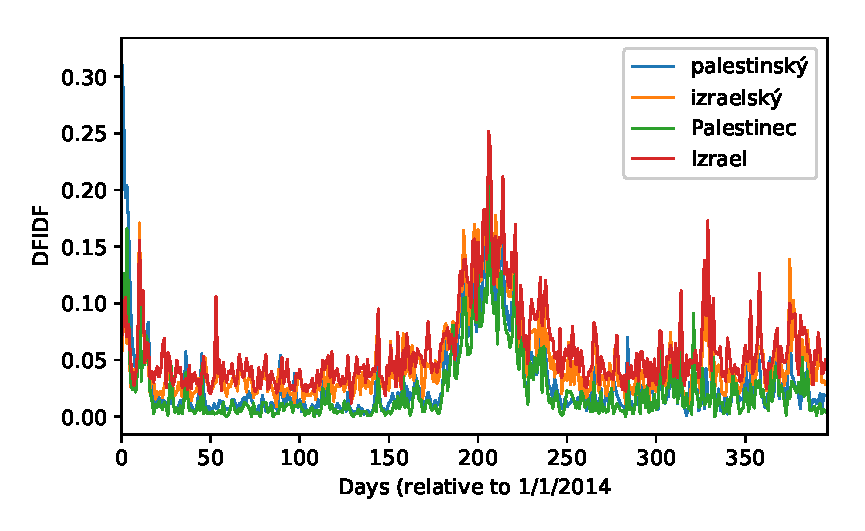
\includegraphics{original_event}  % original event
  \caption{Example of an event detected using the original method. The event consists of the words \textit{palestinian}, \textit{israeli}, \textit{Palestinian} and \textit{Israel}, respectively.}
  \label{fig:original-event}
\end{figure}


\section{Greedy approach}
In this section, we modify the original method to use the Word2Vec model to measure semantic similarity between words. Unlike the document overlap \eqref{eq:document-overlap}, this new similarity measure is able to distinguish semantically similar words even when they do not appear in the same documents. This may happen, for instance, when different authors each use distinct vocabulary when referring to the same event.


\subsection{Semantic similarity}
Some of the astounding results of the Word2Vec model arise from semantically similar words forming clusters \citep{linguistic-regularities} in terms of cosine similarity, which is a standard measure used in information retrieval \citep{information-retrieval, cosine-similarity}.

We replace the document overlap in the cost function \eqref{eq:cost-function-original} by cosine similarity between Word2Vec embeddings, though with a small modification. The cosine similarity is bounded in $[-1, 1]$ with -1 denoting the least degree of similarity. This means that the cost function would reach negative values for highly dissimilar words. This would be a problem, as Algorithm \ref{alg:greedy-event-detection} attempts to minimize it. Consequently, we will transform the cosine similarity into $[0, 1]$, just like the document overlap \eqref{eq:document-overlap}.

The similarity between a set of words $\featset$ and a word $w \notin \featset$ is defined as

\begin{equation}
	\semsim{\featset}{w} = \left( \frac{\inp[\big]{\bar{\embed}_{\featset}}{\embed_{w}}}{\| \bar{\embed}_{\featset} \| \cdot \| \embed_{w} \|} + 1 \right) /\ 2,
\end{equation}

where $\bar{\embed}_{\featset}$ is the mean of all vector embeddings of $\featset$ and $\embed_{w}$ is the vector embedding of $w$. Here, the mean vector virtually represents the central topic of words in $\featset$.


\subsection{Cost function}
We redefine the cost function \eqref{eq:cost-function-original} as

\begin{equation} \label{eq:cost-function}
	\cost{\featset}{w} = \frac{\text{Dist}( \featset \cup w )}{\semsim{\featset}{w} \cdot \sum_{u \in \featset \cup w}{\text{DPS}_{u}}},
\end{equation}

where $\text{Dist}(\cdot)$ is the original trajectory distance function \eqref{eq:trajectory-distance}.

In the original method, \cite{event-detection} defined the cost function \eqref{eq:cost-function-original} for a set of words. However, in Algorithm \ref{alg:greedy-event-detection}, it is always applied on a union of an event constructed so far, and a newly added word. The new cost function must now be applied on such event and word separately due to the nature of Word2Vec similarity definition.

Having constructed the cost function, we use Algorithm \ref{alg:greedy-event-detection} to detect events once again.


\begin{figure}[H]
  \centering
  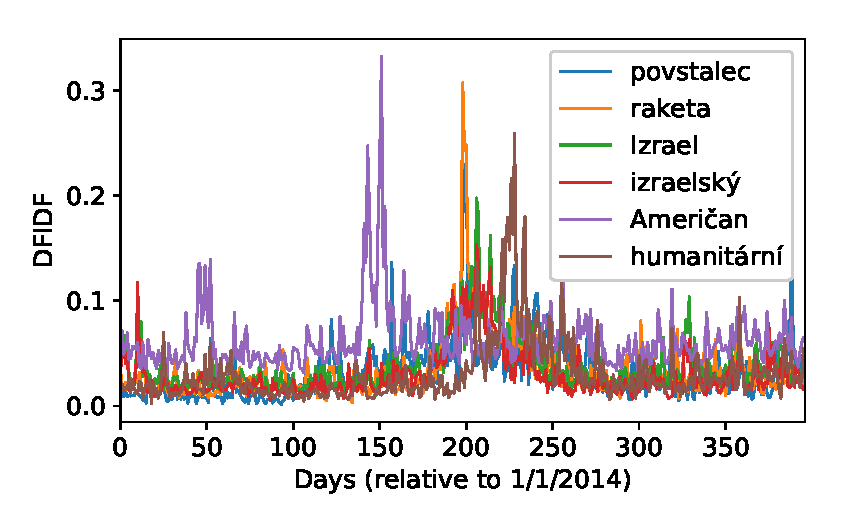
\includegraphics{greedy_event}  % greedy event
  \caption{Example of an event detected using the greedy method. The event consists of the words \textit{to shoot}, \textit{missile}, \textit{Israel} and \textit{israeli}, and is related to the same real event as \autoref{fig:original-event}.}
  \label{fig:greedy-event}
\end{figure}


\section{Cluster-based approach}
Realizing that the keyword-based event detection resembles word clustering, we decided to investigate this idea. In the final method, we apply a clustering algorithm equipped with a custom distance function to the set of eventful words. The distance function is actually a modification of the cost function yet again, though some means have to be taken to make it usable in this context. First, we need to consider a proper clustering algorithm.

The obvious requirement for the clustering algorithm is that it must require no prior knowledge of the desired number of clusters. Another requirement is that the algorithm must accept a custom distance measure.

We considered three candidate algorithms: Affinity propagation \citep{affinity-propagation}, DBSCAN \citep{dbscan} and its modification, HDBSCAN \citep{hdbscan}.

During our experimentation, Affinity propagation performed poorly, its clusters being often seemingly random and of low quality. The quality of HDBSCAN clusters was considerably better, though the algorithm took longer to converge as the number of eventful words grew. It also required to tune multiple parameters, which was difficult to do without any annotated data. We decided to use the DBSCAN algorithm, which outperformed Affinity propagation as well, and does not require to tune as many parameters as HDBSCAN.

In addition to the previously stated requirements, DBSCAN is also capable of filtering out noisy samples (in our case words), not fit for any of the clusters. This property will prove advantageous for our task, as will become clear during the evaluation in \autoref{sec:noise-evaluation}.


\subsection{Noise filtering}
Before we apply clustering, we filter out the noisy parts from the word trajectories. Most words are on some level reported all the time, though only a fraction of these reportings corresponds to notable events. Unlike the greedy optimization described previously, clustering is prone to such noise, and would yield clusters of poor quality, often with trajectories being put together only due to their noisy parts being similar. Additionaly, with DBSCAN capable of filtering out noisy samples, some high quality words could be discarded precisely due to this noise in their (otherwise eventful) trajectories.

We want to keep only those trajectory parts exceeding a certain frequency level, distinguishing notable bursts from the general noise. We do this by computing a cutoff value for each event trajectory and discarding the sectors falling under this cutoff. This procedure is adopted from \cite{online-search-queries}. The algorithm is based on computing a moving average along the trajectory, and works as follows:

\begin{algorithm}[H]
\begin{algorithmic}[1]
\caption{Burst filtering}
\label{alg:burst-filtering}
\Input $\text{window-length} \ l,\ \text{word trajectory} \ \vect{\traj_{w}}$

\State $\vect{MA}_{l} = \text{Moving Average of length} ~ l ~ \text{for} ~ \vect{\traj}_{w} = \left[ \traj_{w}(1), \traj_{w}(2), \dots, \traj_{w}(\streamlen) \right]$

\State $\mathit{cutoff} = \text{mean} \left( \vect{MA}_{l} \right) + \text{std} \left( \vect{MA}_{l} \right)$

\State $\vect{bursts}_{w} = \left[ \traj_{w}(t) \mid \traj_{w	}(t) > \mathit{cutoff} \right]$

\Output $\vect{bursts}_{w}$
\end{algorithmic}
\end{algorithm}


\subsection{Distance function}
We now define the distance function used by DBSCAN. It conveys similar information as the cost function in the previous two algorithms. We still need to measure the trajectory distance as well as semantic similarity between words, though the distance will now be defined strictly pairwise.

For a measure of trajectory distance, we replace the Kullback-Leibler divergence by the Jensen-Shannon divergence JSD \citep{js-divergence-1}, which is symmetric in its arguments. This is a necessary property of the distance function.

Although \cite{event-detection} did symmetrize the Kullback-Leibler divergence, they did not provide any source for their symmetrization form. We were unable to find a case where that particular form was used, though we discovered the Jensen-Shannon divergence, which comes from stronger mathematical background \citep{js-divergence-1, js-divergence-2}. It also tended to improve the clustering quality during our experimentation, as opposed to the original symmetrization. We then decided to replace the original paper's KL-divergence symmetrization by the JS-divergence.

Instead of semantic \textit{similarity}, we measure semantic \textit{distance} as the Euclidean distance between two word vector embeddings. The reason is that Euclidean distance is unbounded, which makes it possible for the samples to be spread farther apart. Since DBSCAN is a density-based clustering algorithm, having high density areas consisting of words with low trajectory distance and similar cosine similarities would cause them to appear in the same cluster. This would cluster the words only in terms of their trajectories, not semantics.

The distance between two words $v$ and $w$ with (normalized and filtered using Algorithm \ref{alg:burst-filtering}) trajectories $\vect{\trajn}_{v},\ \vect{\trajn}_{w}$ and Word2Vec embeddings $\embed_{v},\ \embed_{w}$ is now defined as

\begin{equation}
	\distfunc{v}{w} = \jsd{\vect{\trajn}_{v}}{\vect{\trajn}_{w}} \cdot \| \embed_{v} - \embed_{w}\|_{2},
\end{equation}

with $\jsd{\vect{p}}{\vect{q}} = \frac{1}{2} \left( \kl{\vect{p}}{\vect{m}} + \kl{\vect{q}}{\vect{m}} \right) ,\ \vect{m} = \frac{1}{2} \left( \vect{p} + \vect{q} \right)$.


\subsection{Event detection}
Now, we describe the cluster-based event detection algorithm, which is a direct application of the DBSCAN algorithm and consequent noise filtering.

\begin{algorithm}[H]
\begin{algorithmic}[1]
\caption{Cluster-based event detection}
\Input $\text{Word set EW obtained in \autoref{chap:word-analysis}, matrix } \trajmat \text{, word embeddings for EW}$

\State Precompute a distance matrix $\distmat \in \R^{\left\vert \text{EW} \right\vert \times \left\vert \text{EW} \right\vert}$ with $\distmat_{ij} = \distfunc{w_{i}}{w_{j}}$

\State Apply DBSCAN to $\distmat$, obtaining $k$ clusters and the noisy cluster

\ForEach{$(w, cluster) \in \text{DBSCAN.clusters}$}
	\If{$cluster \neq noise$}
		\State $e_{cluster} = e_{cluster} \cup w$
	\EndIf
\EndFor

\Output $\text{Events} ~ \{ e_{1}, e_{2}, \dots, e_{k} \}$
\end{algorithmic}
\end{algorithm}


\begin{figure}[H]
  \centering
  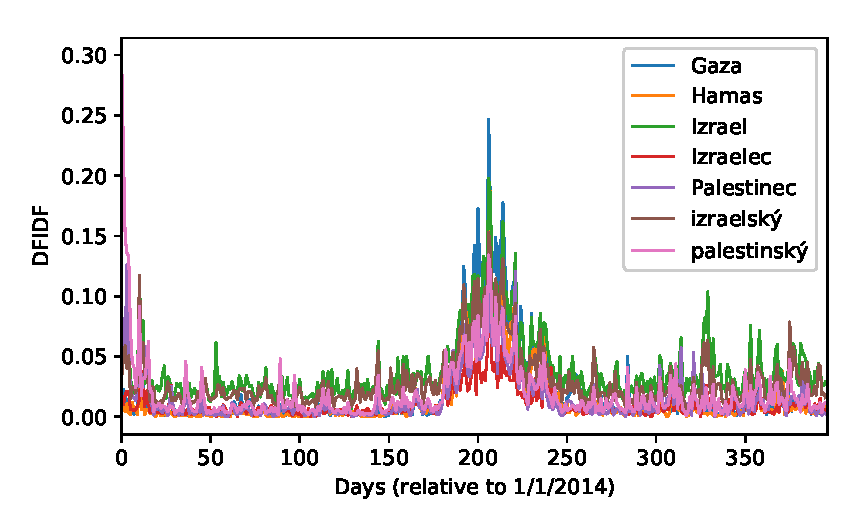
\includegraphics{cluster_event}  % cluster event
  \caption{Example of an event detected using the cluster-based method. The event is related to the same real event as \autoref{fig:original-event} and \autoref{fig:greedy-event}. Note that the trajectories are clear of noise due to application of Algorithm \ref{alg:burst-filtering}}
  \label{fig:cluster-event}
\end{figure}


\chapter{Document retrieval}
\label{chap:document-retrieval}
Having detected the events, we still have to present them to the user in a readable format. A set of keywords may be a concise representation for the computer, but it does not offer much insight into the event itself. We aim to generate short annotations for the events, based on which the user can decide to actually inspect the event more thoroughly and read some of the documents. Consequently, we need to retrieve some number of documents relevant to each event.

We can use each event's temporal and semantic information to query the document collection. The former is trivial -- simply select the documents published within an event's bursty period. The latter will prove more complicated, and we will need to employ some more information retrieval techniques to obtain semantically similar documents.

As of now, an event $e$ is described by a set of its keywords, $\kw{e}$. The goal is to convert this keyword representation to a document representation, $\doc{e}$ of documents related to $e$.

\section{Event burst detection}
First, we need to detect the period when the particular event occurred, so that we can retrieve the documents published around that time. We do this in five steps:

\begin{enumerate}
	\item Construct the event trajectory from the trajectories of its keywords.
	\item Clean the event trajectory.
	\item Determine the event's periodicity.
	\item Fit a probability density function to the event trajectory.
	\item Take the region(s) with the highest density as the bursty period(s).
\end{enumerate}


\subsection{Event trajectory construction}
We will first need to construct an \textit{event trajectory} out of its \textit{keyword trajectories}. We do this by computing a weighted average of the event's keyword trajectories, with weights being the keyword DPS. This ensures that less important words with slightly different time characteristic will not shift the trajectory away from the actual burst.

\begin{equation}
	\vect{\traj_{e}} \coloneqq \frac{1}{\sum_{k \in \kw{e}}{\text{DPS}_{k}}} \sum_{k \in \kw{e}}{\text{DPS}_{k} \cdot \vect{\traj}_{k}}
\end{equation}

{\color{red} TODO: Graph of event keyword trajectories and the weighted average}


\subsection{Trajectory filtering}

Now, a typical event (shown in {\color{red} TODO: Put a pretty picture here}) will usually have some number of dominant bursts corresponding to the period(s) when the event actually occurred. Additionally, there will be some milder, noisy bursts due to the keywords appearing elsewhere, independently of that particular event.

We aim to fit a probability density function to the event trajectory. However, the process would pointlessly try to fit the density to the noisy parts as well as to the bursts. Once again, we apply the Burst filtering algorithm described in \autoref{chap:event-detection} to filter out noise, this time from the event trajectories.

\subsection{Event periodicity}
We apply the signal processing techniques described in \autoref{chap:word-analysis} once more, this time to determine the dominant period $\text{DP}_{e}$ of each event $e$. After obtaining the periodogram, the dominant period is defined as the inverse of the frequency corresponding to the highest peak in the event trajectory:

\begin{equation}
	\text{DP}_{e} \coloneqq \frac{\streamlen}{\argmax\limits_{k \leq \ceil{\streamlen / 2}}{\|X_{k}\|^{2}}}.
\end{equation}

We then consider an event $e$ to be \textit{aperiodic} if it happened only once in the stream, that is if $\text{DP}_{e} > \ceil{\streamlen / 2}$. Similarly, the event is \textit{periodic} if $\text{DP}_{e} \leq \ceil{\streamlen / 2}$.

{\color{red} TODO: Graphs here}

\subsection{Density fitting}
We normalize the event trajectories to have unit sums, so they can be interpreted as probability distribution over days. An element $\traj_{e}(i)$ of the trajectory will denote a probability of that event occurring on day $i$. This allows us to fit a probability density function to them. \cite{event-detection} adapted a similar approach, though only for word rather than event trajectories.

We describe aperiodic and periodic events separately, as different probability distributions must be used in case of a single burst than in case of multiple bursts.

\begin{enumerate}

\item \textbf{Aperiodic events}

An aperiodic event trajectory $\vect{\traj}_{e}$ is modeled by a Gaussian distribution. We fit the Gaussian function

\begin{equation*}
	f(x) = \frac{1}{\sigma \sqrt{2 \pi}} \exp(-\frac{\left( x - \mu \right)^{2}}{2 \sigma^{2}})
\end{equation*}

to the trajectory $\vect{\traj}_{e}$. The parameters $\mu$ and $\sigma$ are estimated using non-linear least squares method. Unlike \cite{event-detection} who use the EM algorithm, least squares proved to be less prone to outliers, yielding a shape more resembling the actual trajectory.

\item \textbf{Periodic events}

A periodic event trajectory $\vect{\traj}_{e}$ is modeled using a mixture of $K = \floor{\streamlen / \text{DP}_{e}}$ Cauchy distributions (as many mixture components as there are periods), as in \cite{health-events}:

\begin{equation*}
	f(x) = \sum_{k = 1}^{K}{\alpha_{k} \frac{1}{\pi} \left( \frac{\gamma_{k}}{\left( x - \mu_{k} \right)^{2} + \gamma_{k}^{2}} \right)}
\end{equation*}

The mixing parameters $\alpha_{k} \geq 0,\ \sum_{k = 1}^{K}{\alpha_{k}} = 1$, location parameters $\mu_{k}$ and scale parameters $\gamma_{k}$ are estimated using the EM algorithm.

The Cauchy distribution has a narrower peak and thicker tails than the Gaussian distribution, which models the periodic bursts more closely. The individual bursts of a periodic event tend to be quite short, but even between two consecutive bursts, the frequency remains at a non-negligible level, which makes the Cauchy distribution a somewhat better choice.

\end{enumerate}


\subsection{Burst detection}
The bursty period of an aperiodic event $e$ is now defined as $\interval{\mu - \sigma}{\mu + \sigma}$. For a periodic event, there are $K = \floor{\streamlen / \text{DP}_{e}}$ bursty periods, each defined as $\interval{\mu_{k} - \gamma_{k}}{\mu_{k} + \gamma_{k}}$.

{\color{red} TODO: More graphs}


\section{Document retrieval}
We only describe the process for aperiodic events. The method is similar for periodic events, except applied on each burst individually.

We need to select some number of documents best representing an event $e$ out of all documents published within the event's bursty period. The only measure of semantics for an event we have is the event's keyword set $\kw{e}$. If we interpret $\kw{e}$ as a keyword query for the document collection, we arrive at the classical task of information retrieval.

In the original method by \cite{event-detection}, the task was simple due to the cost function used. In the paper, the only measure of semantic similarity used was the degree of document overlaps. That way, there was always at least one document in which all of the event's keywords appeared. This is not the case in our method, and we will need to measure the semantic similarity in a more sophisticated way.

There are a few approaches we could take, such as project all documents and queries to a TFIDF space \cite{information-retrieval} and sort the documents by their cosine similarity to the query. This simple approach does not go beyond a trivial keyword occurrence, though after applying some weighting scheme. We could enrich it using Latent Semantic Indexing \cite{lsi} to also take the document topics into account. This would however require us to ``train'' yet another model for this task only, which would be computationally and memory-intensive.

Instead, we decided to further utilize the trained word2vec model and use the recently introduced Word Mover's Distance \cite{wmd}.

The Word Mover's Distance (WMD) is a novel measure of document similarity based on word2vec embeddings of the document words. The similarity of two documents is measured as the minimum distance the word vectors of one document need to ``travel'' to reach the word vectors of the second document.

The WMD discards word order, which makes it suitable for our keyword queries. As the authors note, it achieves best results for short documents, in part due to the method being computationally expensive for larger pieces of text. Therefore, we apply the WMD on document headlines only.

Since the WMD is a measure of distance, we use the WMD similarity instead, defined as

\begin{equation}
	\wmdsim{d_{i}}{d_{j}} \coloneqq \frac{1}{1 + \wmd{d_{i}}{d_{j}}}
\end{equation}

\begin{algorithm}[H]
\begin{algorithmic}[1]
\caption{Document representation of an event}
\Input $\text{Event}\ e,\ \text{number of documents}\ n,\ \text{document stream}\ D$

\State $\mathit{burst\_docs} = \emptyset$

\ForEach{$\mathit{doc} \in D$}
	\If{$\mathit{doc.publication\_date} \in \mathit{e.burst}$}
		\State $\text{Compute}\ \wmdsim{\kw{e}}{\mathit{doc.headline}}$
		\State $\mathit{burst\_docs} = \mathit{burst\_docs} \cup \mathit{doc}$
	\EndIf
\EndFor

\State $\text{Sort}\ \mathit{burst\_docs}\ \text{by the computed}\ \text{Sim}_{\text{WMD}} \ \text{in descending order}$
\Output $\doc{e} = \text{first}\ n\ \text{elements of}\ \mathit{burst\_docs}$
\end{algorithmic}
\end{algorithm}

\chapter{Event annotation}
\label{chap:event-annotation}
The final step of our method is to annotate the detected events in a human-readable way. We aim to generate short summaries so that the user does not have to process a large quantity of text, and can just skim through a few sentences to decide whether he is interested in that particular event. If so, then he can examine the event more closely and go through the actual documents, which we have retrieved in chapter \autoref{chap:document-retrieval}.

Although the keyword set discovered in \autoref{chap:event-detection} provides a concise representation of an event, it can lead to ambiguities or simply not reveal enough information. The keywords should be considered an internal representation used in the detection process, not a feature presentable to the user.

An example of such event whose background is unclear from the keyword set is shown in \autoref{fig:not-recognizable}. After manual examination, we discovered that the event concerns Viktor Yanukovych being ousted from Ukraine's presidency, though it is unclear from the keyword set.


\begin{figure}[H]
  \centering
  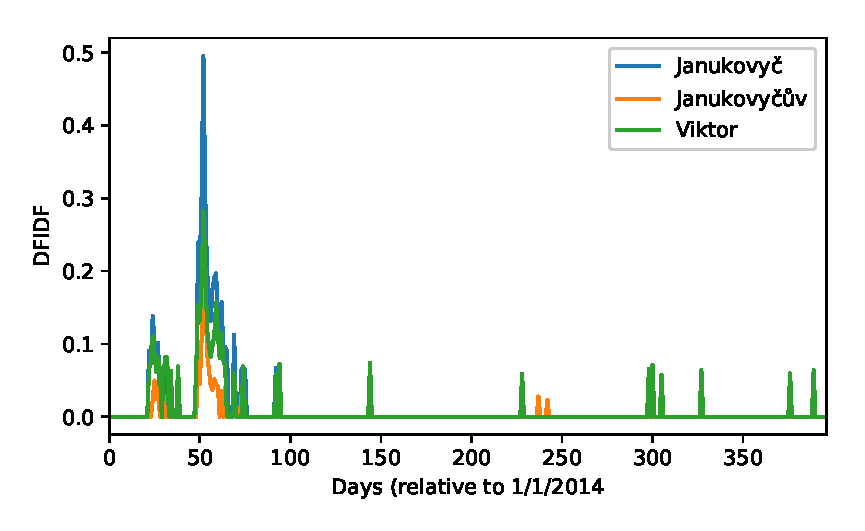
\includegraphics{18_words}  % event not recognizable from its keywords
  \caption{An event whose meaning is not clear from the keyword set.}
  \label{fig:not-recognizable}
\end{figure}


A simple method is to annotate an event by the headline of the most relevant document in terms of Word Mover's Similarity. This may give insight of the general topic of the particular event, but it is unlikely that a whole event will be well characterized by a single document. For this reason, we also investigate a more complex method.

To obtain richer annotations, we apply multi-document summarization techniques to generate a short summary of an event's document set. More specifically, we attempt to extract a subset of sentences out of the event documents, which cover the general topic of the event without providing redundant information. As the documents come from different sources and describe the events from different perspectives, the result will not generally be a continuous paragraph, but more of a set of characteristic sentences. Still, a longer piece of text will likely provide a better insight into an event than a single headline.

We examined the multi-document summarization system presented in \cite{multi-summarization-1, multi-summarization-2}. This system was later improved by \cite{mogren-1}, who evaluated the usage of different word embedding techniques for sentence similarity measures. Their work led to the system presented in \cite{mogren-2} which aggregates several different similarity measures to obtain a better quality summary. We adapt their system and combine together several measures of sentence similarity suitable for the event detection task.


\section{Multi-document summarization}
In \cite{multi-summarization-1}, the authors formulate the task of multi-document summarization as a constrained combinatorial optimization problem, where the goal is to retrieve a subset of sentences maximizing a monotone submodular function $\quality{\cdot}$ measuring the summary quality.

A submodular function $\quality{\cdot}$ on a set of sentences $U$ satisfies the property of \textit{diminishing returns}; that is, for $A \subseteq B \subseteq U \setminus \{ v \},\ \quality{A \cup \{ v \}} - \quality{A} \geq \quality{B \cup \{ v \}} - \quality{B},\ v \in U$. This has an intuitive interpretation for text summarization, namely that adding a sentence $v$ to a longer summary does not improve the summary as much as adding it to a smaller one. The reason is that the information carried by $v$ is likely already present in the longer summary.

Even though solving the task exactly is NP-hard, a greedy algorithm is guaranteed to find a solution only a constant factor off the optimum, as discussed by the authors.

The summary quality is measured in terms of how representative it is to the whole set (coverage) and how dissimilar the sentences are to each other (diversity). The constraints limit the summary to a reasonable length by bounding the total number of words.

In \cite{multi-summarization-1}, basic submodular functions to be used in multi-document summarization are described. In \cite{multi-summarization-2}, these functions are further developed to better capture the semantic properties of sentences.

Mathematically, the task is formulated as

\begin{equation}
\begin{alignedat}{-1}
\max_{S \subseteq U} & \quad \quality{S} = \coverage{S} + \lambda \diversity{S} \\
\text{s. t.} & \quad \sum_{i \in S}{\sentcost_{i}} \leq \budget,
\end{alignedat}
\end{equation}

where $U$ is the set of all sentences from the document set being summarized, $\sentcost_{i}$ is the number of words in sentence $i$ and $\budget$ is the total budget, i.e. the desired maximum summary length.

A feasible set $S$ maximizing $\quality{\cdot}$ will provide a reasonable number of sentences well capturing the overall topic of the whole document set, no two of which being redundant. What remains is to define the coverage function $\coverage{\cdot}$ and diversity function $\diversity{\cdot}$, whose influence can be controlled by the parameter $\lambda \geq 0$. Additionally, the functions must be defined in a way that the submodularity conditions from \cite{multi-summarization-1} are not violated, so that a greedy algorithm can still be used with performance guarantee.


\section{Coverage function}

In \cite{multi-summarization-2}, the coverage function $\coverage{\cdot}$ is defined in terms of pairwise sentence similarity $\semsim{\cdot}{\cdot}$ as

\begin{equation}
\coverage{S} = \sum_{i \in U}{\min{\Big\{ \sum_{j \in S}{\semsim{i}{j}}, \alpha \sum_{j \in U}{\semsim{i}{j}} \Big\} }}.
\end{equation}

The first argument of the minimum measures the similarity between the sentence $i$ and the summary $S$, while the second argument measures the similarity between the sentence $i$ and the rest of the sentences $U$. The number $\alpha \in [0,1]$ is a threshold coefficient controlling the influence of the overall similarity.

In \cite{multi-summarization-1}, the authors further prove that if $\semsim{i}{j} \in [0,1]\ \forall i, j \in U$, the whole function remains submodular.

Originally, only a simple cosine similarity between TFIDF sentence vectors \citep{information-retrieval} was used as $\semsim{\cdot}{\cdot}$. \cite{mogren-1} examined various methods of word embeddings to obtain a finer measure of similarity. This alone outperformed the original method. In \cite{mogren-2}, a more complex system aggregating multiple similarity measures was built, further improving the summary quality. The authors compute the sentence similarity $\semsim{i}{j}$ as a product of these individual similarities, all bounded in $[0, 1]$:

\begin{equation} \label{eq:aggregated-similarity}
	\semsim{i}{j} = \prod_{l}{\similarity_{s_{i}, s_{j}}^{l}}.
\end{equation}

We use this method with several different similarity measures fit for the event detection task. Next, we describe the individual sentence similarities used.

\subsection{TFIDF similarity}

The first measure used is the standard cosine similarity between TFIDF (Term Frequency-Inverse Document Frequency) vectors \citep{information-retrieval} of two sentences $s_{i}$ and $s_{j}$. Such method is a simple measure of document similarity often used in information retrieval.

If we denote the frequency of the word $w$ in sentence $s_{i}$ as $\text{tf}_{w,i}$ and the inverse document frequency of $w$ as $\text{idf}_{w}$, the similarity is written as

\begin{equation}
	\similarity_{s_{i}, s_{j}}^{\mathit{TFIDF}} = \frac{\sum_{w \in s_{i} \cup s_{j}} \text{tf}_{w,i} \cdot \text{tf}_{w,j} \cdot \text{idf}_{w}^{2}}{\sqrt{\sum_{w \in s_{i}} \text{tf}_{w, i}^{2} \cdot \text{idf}_{w}^{2}} \cdot \sqrt{\sum_{w \in s_{j}} \text{tf}_{w, j}^{2} \cdot \text{idf}_{w}^{2}}}.
\end{equation}

The term frequencies are always non-negative, and so the whole cosine similarity is in $[0, 1]$.

The major setback of TFIDF similarity is that it does not go beyond simple word overlap, though weighted to diminish stopwords and amplify important words. That means that if two sentences convey essentially the same information through different vocabulary, they will not be ranked similar due to having only a few words in common. That can be a problem in larger document collections from different sources and authors.

\subsection{Word2Vec similarity}

We attempt to solve this problem by considering the word embeddings of the individual words, as first examined by \cite{mogren-1}.

We represent a sentence $s_{i}$ by summing together the vector embeddings of its words, $\embed_{i} = \sum_{w \in s_{i}} \embed_{w}$. The similarity of two sentences is then the cosine similarity of these vectors, transformed to $[0, 1]$:

\begin{equation}
	\similarity_{s_{i}, s_{j}}^{\mathit{W2V}} = \left(\frac{\inp{\embed_{i}}{\embed_{j}}}{\| \embed_{i} \| \cdot \| \embed_{j} \|} + 1 \right) / \ 2.
\end{equation}

This similarity brings a finer distinction of word-level semantics. This means that even if two sources reporting the same event use fairly different vocabularies, the sentences will still be ranked similar.

\subsection{TR similarity}

The next measure uses Text Rank (TR) similarity, as defined by \cite{textrank}. Each sentence is represented by a set of words, and the overlap of these sets is measured. \cite{mogren-2} achieved best results by combining the TFIDF similarity, word embeddings and the TR similarity, which is defined as

\begin{equation}
	\similarity_{s_{i}, s_{j}}^{\mathit{TR}} = \frac{\left| s_{i} \cap s_{j} \right|}{\log{\left| s_{i} \right|} + \log{\left| s_{j} \right|}}.
\end{equation}


\subsection{Keyword similarity}

In addition to the three previously described similarities, \cite{mogren-2} considered a keyword similarity, which measures the overlap between two sentences and a predefined keyword set. Having previously obtained the event keyword representation $\kw{e}$, we use this measure to make sure the sentences actually concern the particular event.

The similarity is defined as 

\begin{equation}
	\similarity_{s_{i}, s_{j}}^{\mathit{KW}} = \frac{\sum_{w \in \left( s_{i} \cap s_{j} \cap \kw{e} \right)} \text{tf}_{w} \cdot \text{idf}_{w}}{\left| s_{i} \right| + \left| s_{j} \right|}.
\end{equation}

The measure effectively chooses only those sentences having non-zero word overlap with the keyword set. It also breaks the summary fluency, making the summary more of a set of sentences characteristic for the given event. On the other hand, the resulting sentences will be highly relevant to the event, often revealing important information about it.

This tradeoff between fluency and quality is more worth it when summarizing a large number of documents. Even without the keyword similarity, the chance that two summary sentences will make sense consecutively is quite small, when they come from different documents.

If an event consisted of only one or two documents, it would make sense to use a different measure to reach better fluency.

\section{Diversity function}
Now, we can define the diversity function, which will positively reward a summary consisting of non-redundant sentences. \cite{multi-summarization-2} first applied the K-Means clustering algorithm to the TFIDF vectors of the sentences in $U$. The diversity function then positively rewards summaries whose sentences come from different clusters. If the clustering well separates the sentences in the semantic sense, the sentences in different clusters will not carry redundant information.

The diversity function is defined as

\begin{equation} \label{eq:diversity}
	\diversity{S} = \sum_{k = 1}^{K} \sqrt{\sum_{j \in S \cap P_{k}} r_{j}},
\end{equation}

where $P_{k},\ k = 1, \dots, K$ is a clustering of the sentence set $U$. The value $r_{j} = \frac{1}{\left| U \right|} \sum_{i \in U} \similarity_{s_{i}, s_{j}}^{\mathit{TFIDF}}$ is the singleton reward for adding the sentence $i$ into the summary $S$.

This function positively rewards diverse sentences in a sense that once an element $i$ from a cluster $P_{k}$ is chosen, other elements from the same cluster will have diminishing gains due to the square root function (see \cite{multi-summarization-2} for a concrete example). The summarization will then prefer sentences from yet unused clusters.


\section{Optimization}
Having defined the cost function $\quality{\cdot}$, we can use the greedy algorithm defined in \cite{multi-summarization-1} to obtain the desired summary $\annot{e}$ for an event $e$.

For the experiments, we set a budget of 50 words. In the diversity function the number of clusters $K$ was set to $\frac{\left| U \right|}{10}$, putting 10 sentences into each cluster on average. As for the other parameters, we used the values from the original papers \citep{multi-summarization-1, multi-summarization-2}. Additionally, we need to specify which documents we will use for the summarization. In theory, there is no limit to the number of documents, though it would make sense to use only a few most-relevant documents. In \autoref{chap:evaluation}, we will limit the number of documents for efficiency reasons.

\section{Results}
In \autoref{tab:pretty}, we show the annotation for the event depicted in \autoref{fig:not-recognizable}. Though the keywords do not reveal much, the event's topic is fairly clear from the longer summary. We also include the headline of the most relevant document for comparison. In this case, the headline does not provide much insight into the event.

\hspace{\fill}

\begin{tabularx}{\linewidth}{l l} \toprule[1.5pt]
\bf Janukovyč, Janukovyčův, Viktor & \bf (Feb 15 - Mar 2, 2014) \\ \midrule
\multicolumn{2}{p{\linewidth}}{\bf Kdo stojí za Viktorem Janukovyčem?} \\
\multicolumn{2}{p{\linewidth}}{Kyjevská úřadovna prezidenta Viktora Janukovyče je bez stráží. Režim Viktora Janukovyče se zhroutil. Moc ukrajinského prezidenta Viktora Janukovyče se o víkendu zhroutila. Odvolaného ukrajinského prezidenta Viktora Janukovyče stíhá policie. ``Já , Viktor Janukovyč, se obracím na lid Ukrajiny.'' Svržený ukrajinský prezident Viktor Janukovyč se voleb zúčastnit nechce.} \\ \bottomrule[1.25pt]
\caption{Annotation for the event depicted in \autoref{fig:not-recognizable}} \label{tab:pretty}
\end{tabularx}

\hspace{\fill}

In \autoref{tab:ugly}, an event with highly redundant summary is shown. In this summarization, the diversity function \eqref{eq:diversity} failed to diminish similar sentences, and most of the summary simply repeats the same information. On the other hand, the most relevant document's headline represents the event very well, and would suffice to make sense of it.

\hspace{\fill}

\begin{tabularx}{\linewidth}{l l} \toprule[1.5pt]
\bf Adriano, Krnáčová, primátorka & \bf (Oct 12 - Dec 1, 2014) \\ \midrule
\multicolumn{2}{p{\linewidth}}{\bf Pražskou primátorkou bude Adriana Krnáčová z ANO} \\
\multicolumn{2}{p{\linewidth}}{Novou pražskou primátorkou bude Adriana Krnáčová. Primátorkou Prahy bude Adriana Krnáčová (ANO). Novou pražskou primátorkou bude Adriana Krnáčová z ANO. Novou pražskou primátorkou bude Adriana Krnáčová z ANO. Adriana Krnáčová je původem ze Slovenska. Pražskou primátorkou byla zvolena Adriana Krnáčová z hnutí ANO. Bratislavská rodačka Adriana Krnáčová je primátorkou Prahy.} \\ \bottomrule[1.25pt]
\caption{Example of a summary with high degree of redundancy.} \label{tab:ugly}
\end{tabularx}

\hspace{\fill}

Neither of the summaries is fluent enough to be read as an article. In both cases, the summaries resemble unordered sets of sentences, most of which give some insight into the underlying event. The user can stil gain some information from these summaries and consequently decide whether he is interested in the events enough to read the documents.

Further examples of the generated summaries can be found in \autoref{app:clusters-events}.

\chapter{Evaluation}
\label{chap:evaluation}
In this chapter, we compare the three methods for event detection from various standpoints. We will compare the original method (``original''), its modification based on greedy optimization of a different cost function (``greedy'') and the method using clustering algorithm to group similar words together (``cluster'').

Most of these evaluations rate the detected events on the keyword level. We will be referring to the average number of keywords per event, which we provide in the following table.

We discarded trivial events only consisting of a single keyword.

\hspace{\fill}

\begin{minipage}{\linewidth}
\centering
\begin{tabular}{ l c c c }\toprule[1.5pt]
\bf Method 	 & \bf Events detected & \bf Keywords & \bf Keywords per event \\ \midrule
\bf Original & 217 & 451 & 2.08 \\
\bf Greedy   & 82 & 583 & 7.11 \\
\bf Cluster & 77 & 761 & 9.88 \\ \bottomrule[1.25pt]
\end {tabular}\par
\captionof{table}{Average number of keywords per event} \label{tab:title}
\end{minipage}

\hspace{\fill}

\section{Precision, Recall, F-measure}

First, we evaluate precision and recall with respect to a list of real events which occurred during the examined period. The list can be found in \autoref{app:real-events}.

We manually inspected the detected events and matched them with real world events. Out of this assignment, we calculated the precision, recall and F-measure. The results are shown in the table below.

\hspace{\fill}

\begin{minipage}{\linewidth}
\centering
\begin{tabular}{ l c c c }\toprule[1.5pt]
\bf Method 	 & \bf Precision & \bf Recall & \bf F-measure \\ \midrule
\bf Original &  16.35\%     & \bf 28.57\%     &  20.80\% \\
\bf Greedy   &  20.73\%     & 16.33\%      &  18.27\% \\
\bf Cluster &  \bf 25.97\%     & \bf 28.57\%      & \bf 27.21\% \\ \bottomrule[1.25pt]
\end {tabular}\par
\captionof{table}{Precision, Recall and F-measure comparison (manual evaluation)} \label{tab:title}
\end{minipage}

\hspace{\fill}

The original method's precision was poor due to high duplicity of events not appearing in the reference list, which will be more clear in redundancy evaluation later. As the average number of keywords per event is low, the real events are scattered among many detected events. On the other hand, the cluster-based method attained the highest precision due to events consisting of more keywords, meaning lower duplicity.

The greedy method's recall was poor, as the events often consist of unrelated keywords, making them difficult to assign to their real world counterparts.\\

We also attempted to measure precision and recall in a more automatic way, so that the evaluation does not entirely depend on a manual input.

A real event, consisting of occurrence date and a headline, was considered detected if its date was found within a bursty period of some detected event, and if its headline had nonzero intersection with the detected event's keyword set.

\hspace{\fill}

\begin{minipage}{\linewidth}
\centering
\begin{tabular}{ l c c c }\toprule[1.5pt]
\bf Method 	 & \bf Precision & \bf Recall & \bf F-measure \\ \midrule
\bf Original &  7.14\%     & 16.33\%     &  9.94\% \\
\bf Greedy   &  \bf 28.05\%     & \bf 36.73\%      &  \bf 31.81\% \\
\bf Cluster &  20.78\%     & 28.57\%      &  24.06\% \\ \bottomrule[1.25pt]
\end {tabular}\par
\captionof{table}{Precision, Recall and F-measure comparison (automatic evaluation)} \label{tab:title} 
\end{minipage}

\hspace{\fill}

This method of evaluation favors the greedy approach whose keyword sets are less coherent. This allows to intersect a headline more often due to seemingly random words appearing among the keywords. On the other hand, the original method's keyword sets usually consist of only two words that may not appear in the headlines at all.

The cluster-based method's results are similar to the manual evaluation.

\section{Redundancy}

Next, we evaluate redundancy --- the tendency to scatter a real event among several detected events. We manually collected occurrences of the same real event into groups, and computed the redundancy as $1 - (\left| \text{groups} \right| / \left| \text{events} \right|)$.

If it was unclear which real event does a detected event refer to, we considered it to be equal to some other event if they had similar burst characteristics and semantically similar keywords.

\hspace{\fill}

\begin{minipage}{\linewidth}
\centering
\begin{tabular}{ l c }\toprule[1.5pt]
\bf Method 	 & \bf Redundancy \\ \midrule
\bf Original &  77.99\% \\
\bf Greedy   &  75.61\% \\
\bf Cluster &  \bf 42.86\% \\ \bottomrule[1.25pt]
\end {tabular}\par
\captionof{table}{Redundancy comparison} \label{tab:title} 
\end{minipage}

\hspace{\fill}

Large redundancy of the original method is to be expected with events consisting of only 2 keywords on average.

\section{Noisiness}

Next, we evaluate the event noisiness. An event is considered noisy if its trajectory does not contain any distinguishable burst of activity, or if it consists of keywords unrelated to each other. The score is then a fraction of noisy events detected.


\begin{figure}[H]
\centering
\begin{subfigure}{.5\textwidth}
  \centering
  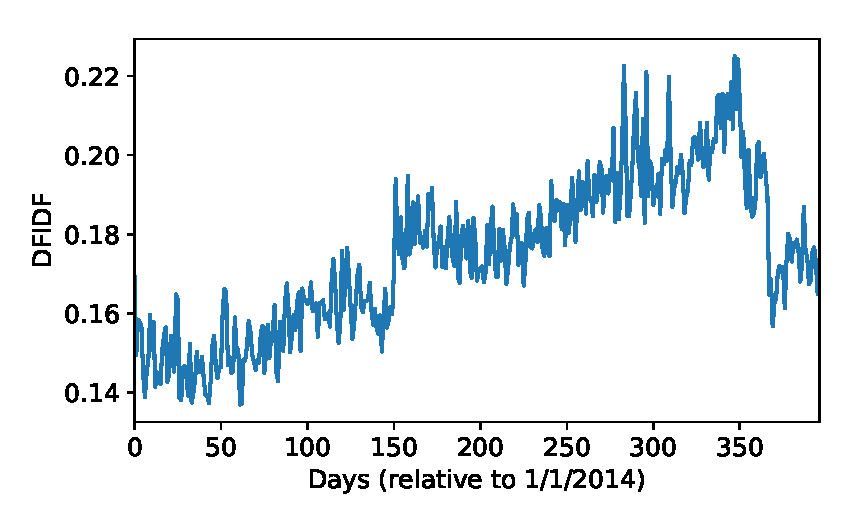
\includegraphics[width=\linewidth]{19_trajectory}  % noisy trajectory
  \caption{Event trajectory}
  \label{fig:noisy-trajectory}
\end{subfigure}%
\begin{subfigure}{.5\textwidth}
  \centering
  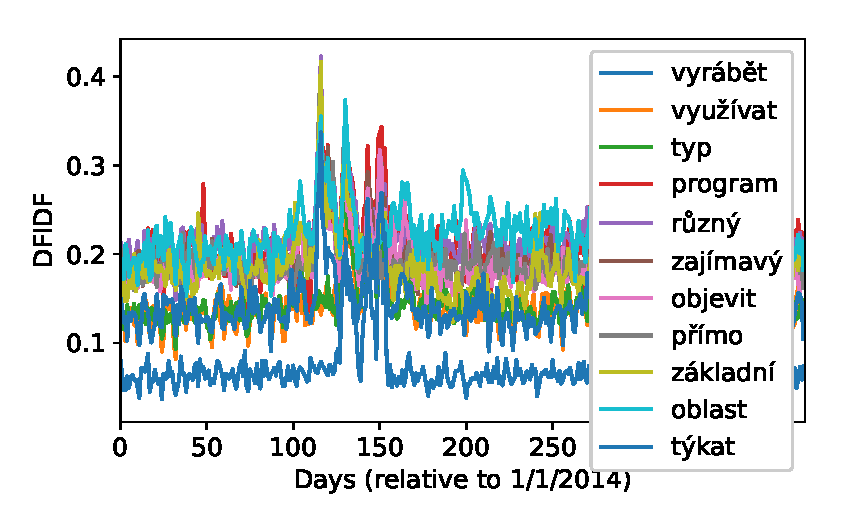
\includegraphics[width=\linewidth]{17_words}  % noisy keywords
  \caption{Event keywords}
  \label{fig:noisy-keywords}
\end{subfigure}
\caption{(a) Event with noisy trajectory. (b) Event with noisy keywords \textit{to make, to utilize, type, program, different, interesting, to discover, directly, basic, area, to concern}.}
\end{figure}


\hspace{\fill}

\begin{minipage}{\linewidth}
\centering
\begin{tabular}{ l c }\toprule[1.5pt]
\bf Method 	 & \bf Noisiness \\ \midrule
\bf Original &  50.94\% \\
\bf Greedy   &  37.80\% \\
\bf Cluster &  \bf 19.48\% \\ \bottomrule[1.25pt]
\end {tabular}\par
\captionof{table}{Noisiness comparison} \label{tab:title} 
\end{minipage}

\hspace{\fill}

Here, the cluster-based method performed the best, as the clustering algorithm chosen (DBSCAN) is capable of automatic filtering of noisy samples. With the distance function measuring both trajectory and keyword similarity, it filters out words unrelated to any event.

Poor performance of the original method is partially caused by its large redundancy. Even if a number of words with noisy trajectories appears in similar documents, the method would not group them together to a single event, but split into several noisy events. All of these noisy events then negatively contribute to the noisiness score.

Surprisingly, the greedy method did not perform the worst even though manual check revealed poor keyword quality {\color{red} TODO: As can be seen from the purity evaluation?}. This can again be explained by larger keyword sets of the greedy method, which makes even the noisy words clustered together into a smaller number of noisy events.

\newpage

\section{Purity}

All previous evaluations concerned the events on the keyword level. The purity measure will evaluate the event document sets in terms of topical consistency. This is a metric used by \cite{document-purity}.

The evaluation is similar to the standard measure of cluster purity in the sense that we measure the consistency of class labelling within each cluster. Each event is interpreted as a cluster of documents. Clearly, a high quality event should contain documents concerning similar topics. The problem is that our documents do not have any notion of class labels, which we will have to supplement.

We first assembled a list of 50 words from 1000 most often occurring Nouns and Verbs in document headlines. The words are \textit{Ukrajina (Ukraine), Rusko (Russia), policie (police), soud (court), Zeman, EU, Sparta, festival, Babiš, Putin, Google, ekonomika (economics), letadlo (airplane), východ (east), politika (politics), zabít (to kill), poslanec (deputy), armáda (army), Kyjev (Kiev), Škoda, hokejista (hockey player), fotbalista (football player), doprava (traffic), vražda (murder), Vánoce (Christmas), Francie (France), sport, NATO, Moskva (Moscow), ropa (petroleum), turnaj (tournament), Obama, referendum, ebola, parlament (parliament), koalice (coalition), Paříž (Paris), automobil, mistrovství (championship), elektrárna (power plant), Sýrie (Syria), islamista (islamist), Brusel (Brussels), olympiáda (olympics), sníh (snow), průmysl (industry), revoluce (revolution), výbuch (explosion), finance, terorista (terrorist)}. All documents that contained any of these words in their headline were tagged with the corresponding class label.

Then, for each event, we computed the fraction of documents with the most frequently appearing class label out of all tagged documents. The measure is a weighted average of these values across all events, with weights being the number of tagged documents within each event.

\hspace{\fill}

\begin{minipage}{\linewidth}
\centering
\begin{tabular}{ l c }\toprule[1.5pt]
\bf Method 	 & \bf Purity \\ \midrule
\bf Original &  30.53\% \\
\bf Greedy   &  {\color{red} TODO} \\
\bf Cluster &  \bf 61.08\% \\ \bottomrule[1.25pt]
\end {tabular}\par
\captionof{table}{Purity comparison} \label{tab:title} 
\end{minipage}

\hspace{\fill}

\section{Computation time}

Finally, we evaluate the computation time. We measure the execution time of the individual detection steps, so it is clear which parts are the bottlenecks. All experiments were performed on a laptop computer with a 64bit operating system, quad-core processor and 8GB RAM.

\hspace{\fill}

\begin{minipage}{\linewidth}
\centering
\begin{tabular}{ r c c c }\toprule[1.5pt]
\bf Unit & \bf Original & \bf Greedy & \bf Clusters \\ \midrule
Word2Vec embedding & --- & \multicolumn{2}{c}{3h 50min} \\
Bag of words model construction & \multicolumn{3}{c}{37min} \\
Word trajectories \& spectral analysis & \multicolumn{3}{c}{8s} \\
Event detection & 2min 12s & 50s & 4min 50s \\
Document retrieval & 7min 30s & {\color{red} TODO} & 7h 40min \\
Event annotation & {\color{red} TODO} & {\color{red} TODO} & {\color{red} TODO} \\ \midrule
\bf Total & & & \\ \bottomrule[1.25pt]

\end{tabular}\par
\captionof{table}{Computation time comparison} \label{tab:title}
\end{minipage}

\hspace{\fill}

{\color{red} TODO: Measure how much of the BOW model construction is taken by IO operations.}

{\color{red} TODO: Write a conclusion of this evaluation once the results are known.}



\chapter{Conclusion}
\label{chap:conclusion}
We examined how event detection methods depending on keyword representation could be improved by considering word embedding models, namely the Word2Vec model \citep{word2vec}. We tried to augment an existing method by \cite{event-detection} to use a Word2Vec-based similarity function to match semantically related words together. This did not bring significant improvement -- although the detected events were richer and less redundant, a notable amount of noise appeared. This made the events hard to assign to their real world counterparts, as most of their keywords did not contribute to any underlying topic.

Then, we explored a different approach, where we interpreted the keyword-based event detection as a literal clustering task. We defined a custom distance function also utilizing the Word2Vec model as a semantic measure. We then applied a clustering algorithm equipped with this distance function to words previously selected as eventful. Our evaluation suggests that this method was more successful than both the original method and its Word2Vec modification. The resulting events were composed mostly of representative words and reached lesser redundancy and noisiness than the previous methods.

The disadvantage of both our methods is the necessity to train the Word2Vec model, which is time consuming. However, it can be trained once and than reused for subsequent detections, as long as the document vocabulary remains similar.

We also examined how the Word2Vec model could be used to retrieve documents concerning the detected events. We applied the Word Mover's Distance \citep{wmd} to documents within each event's bursty period as a measure of their relevance to that particular event's keyword set. We then selected the most relevant documents as the event's document representation. Although the documents were of high quality and represented the events well, the process took an unbearable amount of time. In the original method, the retrieval process was more straightforward and much more efficient.

Finally, we applied multi-document summarization techniques to the documents to obtain a short summary describing each event. This, along with the event's occurrence dates and document sets, are the outputs of our method presented to the user. The summaries serve the purpose of giving a quick reference of the event's topic, based on which the user may decide to examine the event further and go through the retrieved documents.

In future work, it would be beneficial to use a more efficient way of computing the documents relevant to each event. Traditional information retrieval techniques, such as Latent Semantic Indexing \citep{lsi} could be used here, perhaps with some domain specific knowledge of the underlying events, such as their bursty periods.

Also, we would like to examine how an event could be represented directly as a set of documents, rather than words. Although there are attempts to do so \citep{document-bursty-representation}, they require to fine-tune a number of parameters, and the document representation is again constructed using word trajectories. The Doc2Vec model \citep{doc2vec}, a generalization of Word2Vec able to embed whole documents in a vector space, could be used to obtain the semantic representation.

Instead of computing a cutoff value to clean a word or an event trajectory, as we did in \autoref{chap:event-detection}, further signal processing techniques could be applied on the trajectories to separate the dominant bursts from the underlying noise. The result would be a somewhat cleaner trajectory devoid of any milder bursts of no interest. This could lower the noisiness, since words would be matched together based on only the dominant activity, not any underlying influence, which still eludes the cutoff value method.


% Appendices
\appendix
\chapter{List of real events used for evaluation}
\label{app:real-events}
This is a list of confirmed events which occurred in 2014 that was used to evaluate Precision and Recall.

\begin{tabularx}{\linewidth}{@{}c @{}c X@{}}\toprule[1.5pt]
\bf \# & \bf Date & \bf Headline \\ \midrule
1 & June 2 & Španělský král Juan Carlos I. abdikoval a za svého nástupce určil svého syna Filipa. \\ \midrule
2 & June 4-5 & Konal se 40. summit G8 v Bruselu. \\ \midrule
3 & June 7 & Petro Porošenko složil prezidentskou přísahu a stal se prezidentem Ukrajiny. \\ \midrule
4 & June 8 & Abd al-Fattáh as-Sísí složil prezidentskou přísahu a stal se prezidentem Egypta. \\ \midrule
5 & June 10 & V izraelských prezidentských volbách byl zvolen Re'uven Rivlin. \\ \midrule
6 & June 12 & V Brazílii začalo 20. mistrovství světa ve fotbale. \\ \midrule
7 & June 15 & Andrej Kiska složil prezidentskou přísahu a stal se prezidentem Slovenska. \\ \midrule
8 & June 18 & Vůdci vojenského převratu v Turecku z roku 1980 Kenan Evren a Tahsin Şahinkaya byli odsouzeni na doživotí. \\ \midrule
9 & June 19 & Filip, asturský kníže složil přísahu a stal se králem Španělska jako Filip VI. Španělský \\ \midrule
10 & July 1 & Itálie se ujala předsednictví EU. \\ \midrule
11 & July 8 & Armáda České republiky utrpěla největší ztrátu v novodobých dějinách, kdy při sebevražedném útoku poblíž letecké základny Bagram zemřeli čtyři čeští vojáci, spolu s dalšími 12 tamními oběťmi. Pátý český voják byl těžce raněn a 14. července zemřel. \\ \midrule
12 & July 13 & Mistry světa ve fotbale se stala německá fotbalová reprezentace. \\ \midrule
13 & July 15 & Novým předsedou Evropské komise se stal lucemburský politik a bývalý premiér Jean-Claude Juncker. \\ \midrule
14 & July 17 & V oblasti bojů na východní Ukrajině se zřítil Boeing 777 malajsijských aerolinií. Zemřelo všech 295 osob na palubě. \\ \midrule
15 & July 21 & Vláda Bohuslava Sobotky vybrala nového eurokomisaře. Stane se jím ministryně pro místní rozvoj Věra Jourová, která ve výběru porazila Pavla Mertlíka. \\ \midrule
16 & August 10 & V historicky první přímé prezidentské volbě v Turecku byl zvolen premiér Recep Tayyip Erdoğan. \\ \midrule
17 & August 16-28 & Letní olympijské hry mládeže 2014 v čínském Nankingu. \\ \midrule
18 & August 19 & Americký novinář James Foley byl popraven v syrské poušti neznámým islámským radikálem, jeho smrt vyvolala v západním světe vlnu pobouření. \\ \midrule
19 & August 24 & Meziplanetární sonda New Horizons prolétla blízko L5 soustavy Slunce–Neptun. \\ \midrule
20 & August 25 & Ve sporu o amnestii Václava Klause soud schválil smír, podle něhož se bývalý hradní právník Pavel Hasenkopf na vyhlášeném znění amnestie nepodílel. \\ \midrule
21 & August 28 & Recep Tayyip Erdoğan složil prezidentskou přísahu a stal se prezidentem Turecka. \\ \midrule
22 & August 30 & Polský premiér Donald Tusk byl na summitu Evropské unie zvolen předsedou Evropské rady. \\ \midrule
23 & September 1 & Pavel Hasenkopf podal na Vratislava Mynáře trestní oznámení pro pomluvu ohledně Mynářova výroku, že Hasenkopf je jedním z autorů amnestie Václava Klause. \\ \midrule
24 & September 2 & Další americký novinář Steven Sotloff byl popraven v syrské poušti neznámým islámským radikálem, stejně jako James Foley v srpnu. \\ \midrule
25 & September 4 & Ve Vilémově se zřítil most, na kterém probíhala rekonstrukce. Zemřeli čtyři dělníci, další dva byli zraněni. \\ \midrule
26 & September 6 & Počet nakažených ebolou při celoroční epidemii se přehoupl přes 4 000. \\ \midrule
27 & September 8 & Britský následník trůnu Princ William a jeho manželka Kate oznámili, že čekají druhé dítě. \\ \midrule
28 & September 10 & Kandidátka na českou eurokomisařku Věra Jourová získala portfolio spravedlnosti, spotřebitelské politiky a rovnosti pohlaví. \\ \midrule
29 & September 13 & Islámští radikálové popravili dalšího západního zajatce, tentokrát jím byl britský humanitární pracovník David Haines. \\ \midrule
30 & September 18 & Ve Skotsku proběhlo referendum o nezávislosti na Spojeném království. Pro odtržení od Británie hlasovalo 44,7\% lidí, proti 55,3\% lidí, Skotsko tak zůstane její součástí. \\ \midrule
31 & September 20 & Náčelník Generálního štábu Armády ČR Petr Pavel byl zvolen předsedou vojenského výboru NATO. \\ \midrule
32 & September 24 & Na Pražský hrad se dostal výhružný dopis adresovaný prezidentovi Miloši Zemanovi s bílým práškem. Případ šetří policie. \\ \midrule
33 & October 3 & Prezident Miloš Zeman přijal demisi ministryně pro místní rozvoj Věry Jourové. \\ \midrule
34 & October 3 & Islámští radikálové popravili dalšího západního zajatce, stal se jím opět britský humanitární pracovník Alan Henning. \\ \midrule
35 & October 7 & Evropský parlament schválil nominaci Věry Jourové na post eurokomisařky pro spravedlnost, spotřebitelskou politiku a rovnost pohlaví. \\ \midrule
36 & October 10-11 & Proběhly volby do Senátu Parlamentu České republiky, volby do zastupitelstev obcí a volby do Zastupitelstva hlavního města Prahy. Ve volbách uspěly především vládní strany ČSSD, ANO a KDU-ČSL. \\ \midrule
37 & October 14 & Žena trpící schizofrenii pobodala na obchodní akademii ve Žďáru nad Sázavou tři studenty a zasahujícího policistu. Jeden ze studentů útok nepřežil. \\ \midrule
38 & October 16 & Ve Vrběticích došlo k výbuchu muničního skladu č. 16. Na místě zahynuli dva zaměstnanci skladu, došlo k evakuaci obyvatel přilehlých obcí. \\ \midrule
39 & October 16 & Zanikla europarlamentní frakce Evropa svobody a přímé demokracie, 20. října byla opět obnovena. \\ \midrule
40 & October 17-18 & Proběhlo druhé kolo voleb do Senátu Parlamentu České republiky. Ve volbách uspěly především vládní strany ČSSD, ANO a KDU-ČSL. \\ \midrule
41 & November 9 & V Katalánsku začalo symbolické hlasování o nezávislosti na Španělsku. \\ \midrule
42 & November 12 & Přistál modul Philae jako historicky první lidský stroj na kometě. \\ \midrule
43 & November 15 & Islámští radikálové popravili dalšího západního zajatce, stal se jím americký humanitární pracovník Peter Kassig. \\ \midrule
44 & November 15-16 & Summit G20 v Brisbane. \\ \midrule
45 & December 1 & Ledovková kalamita ochromila hromadnou dopravu v ČR a dodávky elektřiny v mnoha regionech. Tramvajová doprava v Praze dokonce poprvé ve své historii zažila úplné zastavení provozu. Do normálu se dopravní i energetická situace vrátila až 3. prosince. \\ \midrule
46 & December 1 & Druhým předsedou Evropské rady se stal Donald Tusk. \\ \midrule
47 & December 3 & Ve Vrběticích došlo k dalšímu výbuchu muničního skladu č. 12. Opět proběhla evakuace obyvatel přilehlých obcí, oba dva výbuchy jsou vyšetřovány jako úmyslný trestný čin. \\ \midrule
48 & December 16 & Ozbrojenci ze skupiny Tahrík-e Tálibán-e Pákistán spáchali masakr v péšávarské vojenské škole škole. Útok si vyžádal 141 obětí většinu z nich tvořili děti. \\ \midrule
49 & December 28 & Na cestě ze Surabaje do Singapuru se ztratilo letadlo malajsijské společnosti AirAsia se 162 lidmi na palubě. \\

\bottomrule[1.25pt]
\end{tabularx}

\chapter{Events detected using the cluster-based method}
\label{app:clusters-events}
\begin{tabularx}{\linewidth}{r m{2.5cm} X m{8cm}}\toprule[1.5pt]
\bf \# & \bf Keywords & \bf Burst & \bf Summary \\ \midrule

1 & Adaptive, Direct, Eija, Golf, Hama, Harmonious, Infiniti, Japonec... & May 23 - Jun 4, 2014 & Audi A 3 clubsport quattro concept vychází z modulární platformy MQB pro vozy s motorem uloženým vpředu napříč. Také profil limuzíny má ostřejší charakter. Příď vozu je vyrobena z oceli. Vzhled exteriéru zatím zůstává tajemstvím. Předchůdce byl nabízen pouze s pětidveřovou karoserií. \\ \midrule
2 & Adriano, Krnáčová, primátorka & Oct 12 - Dec 1, 2014 & Novou pražskou primátorkou bude Adriana Krnáčová. Primátorkou Prahy bude Adriana Krnáčová (ANO). Novou pražskou primátorkou bude Adriana Krnáčová z ANO. Novou pražskou primátorkou bude Adriana Krnáčová z ANO. Adriana Krnáčová je původem ze Slovenska. Bratislavská rodačka Adriana Krnáčová je primátorkou Prahy. \\ \midrule
3 & Alta, Celerio, funkčnost, rozvora, sázející, udávat, užitný & Apr 10 - May 8, 2014 & S délkou 3,6m je Celerio o 10cm delší nežli aktuálně nejmenší Suzuki Alto, rozvor náprav měří 2,42m a objem jeho zavazadelníku udává výrobce 254l. Při zkoušce funkčnosti výtahu zemřel. Tempo Nexusu 6 má udávat osmijádrový čipset MediaTek. \\ \midrule
4 & Andrej, Babiš & Jan 17 - Feb 11, 2014 & Dá se něco takového vytknout Andreji Babišovi? Příspěvek Andrej Babiš pochází z Borovan.cz. Andrej Babiš také přinesl do politiky nový vítr. Andrej Babiš je kouzelník na slovo vzatý. ODS: Andrej Babiš by měl rezignovat. Novými náměstky Andreje Babiše jsou Wagenknecht a Hornochová. \\ \midrule
4 & Andrej, Babiš & Mar 25 - Apr 10, 2014 & Andrej Babiš to nemá lehké. Co se děje v hlavě Andreje Babiše? A když to Babiš neprosadí? Andreje Babiše, v níž nemůže zvítězit. Šokující, ministr financí Andrej Babiš jde proti nemocným?! Zpřísníme jejich postihy, uvedl ministr financí Andrej Babiš. \\ \midrule
4 & Andrej, Babiš & May 20 - Jun 30, 2014 & Jak by se choval Andrej Babiš? Andrej Babiš se v televizi rozpovídal. Ale pokutu prý za něj zaplatí Andrej Babiš. Co vám to sděluje Andrej Babiš? Andrej Babiš, psáno pro Lidové noviny. Andrej Babiš se prý bojí Miroslava Kalouska. \\ \midrule
4 & Andrej, Babiš & Jul 7 - Aug 25, 2014 & Co vám to sděluje Andrej Babiš? Možná na tom má svůj podíl její předseda, Andrej Babiš. Šestici uvedl předseda hnutí Andrej Babiš. Neaktuálně: O co byl okraden Andrej Babiš? Sobotka je s Babišem spokojen. Andrej Babiš, psáno pro Hospodářské noviny. \\ \midrule
4 & Andrej, Babiš & Oct 3 - Oct 20, 2014 & Není to úspěch nějakého politického hnutí, ale úspěch Andreje Babiše. Nezapomínejme na Andreje Babiše, který to celé přikrývá. A tou je Andrej Babiš. Andrej Babiš není standardní politik. Přesto Andrej Babiš u voličů boduje. O legálnosti majetku Andreje Babiše žádné pochybnosti nemám. \\ \midrule
4 & Andrej, Babiš & Oct 25 - Jan 4, 2015 & Mládek s Babišem se nedohodli. Inu, ale i to je styl Andreje Babiše. Tu potvrdil i ministr Babiš. Andrej Babiš se může pochlubit skutečně jen panem ministrem Stropnickým. I Babiš už je politikem. Celý projev ministra financí Andreje Babiše si můžete přečíst zde. \\ \midrule
5 & Audi, Bosch, Championship, Citroen, Civic, Climawork, DOHC, Daimler... & Apr 22 - May 11, 2014 & Toyota Yaris Hybrid patří mezi nejoblíbenější hybridní modely značky Toyota. Foto: Toyota. Lamborghini Urus by mohlo být prvním modelem automobilky s přeplňovaným motorem. Spalovací motor Toyota FPEG je určen výhradně vozům s hybridním pohonem. Nový třílitrový turbodiesel Audi přináší vyšší výkon a nižší spotřebu. \\ \midrule
6 & Australian, Melbourne & Jan 7 - Feb 3, 2014 & Australian Open začne v pondělí. V Melbourne právě probíhá los Australian Open. Melbourne - Tenista Tomáš Berdych postoupil do druhého kola grandslamového Australian Open. Melbourne - Český tenista Tomáš Berdych postoupil do třetího kola grandslamového Australian Open. Berdych si v Melbourne ve finále nezahraje. \\ \midrule
7 & Bagdád, Irák, irácký & Jun 26 - Sep 10, 2014 & V Bagdádu má Hague jednat s iráckým premiérem Núrím Málikím. Britský ministr zahraničí Hague přicestoval do Bagdádu. Ruské Su - 25 pro Irák Cílem povstalců je dobytí Bagdádu. Islamisté postupují od června severním Irákem směrem k Bagdádu. Radikálové z IS postupují Irákem. \\ \midrule
8 & Bartošová, Iveta, Rychtář & Apr 29 - May 6, 2014 & Přijde Iveta Bartošová o dům? Kdo je vrahem Ivety Bartošové? Iveta Bartošová včera spáchala sebevraždu. Smrt Ivety Bartošové nebyla náhodná? Iveta Bartošová raději zvolila smrt. Josefu Rychtáři hrozí obvinění kvůli sebevraždě Ivety Bartošové. Příbuzní Ivety Bartošové se spojili proti Josefu Rychtářovi. \\ \midrule
8 & Bartošová, Iveta, Rychtář & May 7 - May 16, 2014 & Josef Rychtář je podezřelý z účasti na sebevraždě Ivety Bartošové. POLICIE PODEZÍRÁ RYCHTÁŘE z podílu na sebevraždě Ivety Bartošové! Policie podezírá Josefa Rychtáře ze spoluúčasti na sebevraždě Ivety Bartošové. Josef Rychtář pozval rodinu Ivety Bartošové prostřednictvím SMSky. Pohřeb Ivety Bartošové byl bez jejích nejbližších. \\ \midrule
8 & Bartošová, Iveta, Rychtář & Jan 9 - Jan 11, 2015 & Rychtář raboval ve vile Ivety Bartošové! Tu ale Rychtář zpravodajství Primy vystavit nehodlá. Ví něco o zubech Ivety, co neví Macura? Exkluzivně: Máme poslední telefonát Bartošové! Žhavé drby.Alice Bendová: Chystá druhou svatbu! Vdovec po Ivetě Bartošové řeší další nepříjemnost! \\ \midrule
9 & Betlém, Ježíšek, Vánoce, advent, adventní, betlém, cukroví, dárek... & Dec 5 - Dec 31, 2014 & Co si odnesete: Sadu 6ks originálních vánočních ozdob na stromeček. Použila jsem stromečky a domy. Vánoční stromek je nepostradatelnou součástí Vánoc. Advent by měl býti časem zamyšlení. Vánoční kapr není hotový za jeden rok. Bez vánočního stromku si nikdo Vánoce nedokáže představit. \\ \midrule
10 & Brazílie, brazilský & Jun 10 - Jul 12, 2014 & Fotbalové MS vyhraje podle bookmakerů Brazílie. Metropolí Brazílie je město Brasília. Pochválil tak za výdrž brazilského mladíka. Paraguay a Brazílii trápí povodně. ``Těžko jsme hledali cestu k brazilské brance.'' Nehrají ten klasický pohledný brazilský fotbal. Brazilský záložník Diego se upsal Fenerbahçe. \\ \midrule
11 & Brémy, CNG, Citigo, Combi, Corporation, DIG, Designwork, Ecoboost... & Jun 5 - Jun 12, 2014 & Elektromobil Mercedesu odstartoval v Kalifornii. Automobilka Mercedes-Benz se s vývojem svého elektromobilu postaveného na třídě B přestěhovala do kalifornského centra v Sunnyvale. Japonská automobilka Mitsubishi Motors Corp. je hodně aktivní v předvádění koncepčních vozů, které se prezentují na významných... \\ \midrule
11 & Brémy, CNG, Citigo, Combi, Corporation, DIG, Designwork, Ecoboost... & Jun 13 - Jun 18, 2014 & Dvoudílný koncept skříně byl zachován. Kombi je lepší, ale ne o moc. Minimálně už v prvním Focusu byla přesně ta samá. Tým bude tvořen 150 inženýry a designéry. Aktuálně jsme informovali o jednání BMW a Tesla Motors týkajících se spolupráce v oblasti dobíjení elektromobilů. \\ \midrule
12 & Charlie, Hebdo, Mohamed, Paříž, islám, karikatura, muslim, muslimský... & Jan 6 - Jan 17, 2015 & V redakci satirického listu Charlie Hebdo v Paříži se střílelo. Prorok Mohamed: Já jsem Charlie. Oběti útoku uctila také Paříž. Muslimský svět protestuje proti karikaturám v Charlie Hebdo. Demonstrace proti karikaturám proroka Mohameda v pákistánském Karáčí. Mstili se údajně za karikatury Mohameda. \\ \midrule
13 & China, Cross, Ostřihom, Peking, SUV, Suzuki, Transporter, Volkswagen... & May 10 - Jun 1, 2014 & VW užitkové vozy si poradí i s mimořádně extrémním terénem. A absolutní jedničkou jsou... Zatímco automobilová Evropa se jenom pomalu zvedá ze dna, láká Říše středu stále ještě snovými dvoucifernými nárůsty prodeje. Decentně navýšená světlost vozu a krátké převisy jsou typické pro SUV. \\ \midrule
14 & Dakar, Loprais & Dec 28 - Jan 24, 2015 & Společně hledíme několik let dopředu. Čísla ale na Dakaru kolikrát nic neznamenají. Takovou rychlostí na Rallye Dakar ještě nejel. Šestý Aleš Loprais je o dalších 29 sekund zpět. Mardějevův skalp získali tentokrát i Kolomý s Lopraisem. Španěl Marc Coma vyhrál Dakar už pětkrát. \\ \midrule
15 & Ebola, Guinea, Leone, Libérie, Sierra, ebola, epidemie & Sep 28 - Oct 29, 2014 & Ebola nejdříve propukla v Guineji. Nejvíce postižené země jsou Sierra Leone, Guinea a Libérie. Libérie je spolu se Sierrou Leone a Guineou nejpostiženější ze západoafrických zemí. Zatím epidemie eboly hlavně postihovala východ Sierra Leone. WHO: Epidemie eboly v Libérii začala ustupovat. \\ \midrule
16 & Ford, elektromobil & Apr 9 - Apr 12, 2014 & Ford se snaží dohnat, co se dá. Že elektromobily nemají u nás na růžích ustláno, není nic nového. Elektromobil bude mít brzy každá automobilka. Volkswagen zahájil předprodej svého prvního elektromobilu na českém trh. V Třinci vznikla dobíjecí stanice pro elektromobily. \\ \midrule
16 & Ford, elektromobil & Apr 12 - Apr 17, 2014 & Mercedes-Benz třídy B jako elektromobil už se testuje. Vyhledat vozidla v inzerci: Ford. Henry Ford se nemohl dočkat rána. Ford ale svou pásovou výrobu rovněž hájil. V roce 1903 založil Motor Ford Company. Ford Mustang slaví padesátku výročním modelem. \\ \midrule
16 & Ford, elektromobil & Apr 19 - Apr 22, 2014 & Moc technických informací samozřejmě nemáme. Osobně jsem fanoušek značky Ford. Kde tedy koupit výhodně v Praze Ford? Ford Praha má na výběr všechny modely. Prvním elektromobilem od BMW byl stroj založený na kupé 1602. Ford nebude tento doplněk nabízet pro jiné Mustangy. \\ \midrule
16 & Ford, elektromobil & Jun 3 - Jun 5, 2014 & BMW dodalo první elektromobily ActiveE do USA. Automobilka BMW nechala v USA sešrotovat minimálně desítky testovacích elektromobilů ActiveE. Ford rozdělí 500 nových Mustangů mezi 20 zemí. Odlehčené komponenty srazily hmotnost Fordu Fusion o 25 procent. VIDEO: elektromobil BMW i 3 umí zaparkovat sám. \\ \midrule
16 & Ford, elektromobil & Jun 6 - Jun 12, 2014 & Jaký tedy Ford Kuga je? Její vedoucí představitelé se obrátili na Ford. Že vám elektromobily zrovna nevoní? Elektromobil Mercedesu odstartoval v Kalifornii. Vozy BMW a Ford se budou prohánět v Hradci. Ford Fiesta je nejprodávanějším modelem Fordu v Evropě. \\ \midrule
16 & Ford, elektromobil & Jun 13 - Jun 18, 2014 & Fiesta je nejprodávanějším modelem Fordu v Evropě. Elektromobil Mercedesu odstartoval v Kalifornii. Zpočátku se počítá s výrobou 5 000 elektromobilů ročně. Tabulky hmotnosti údajně zveřejnil jeden z amerických dealerů Fordu. Takový je Ford Fiesta s převodovkou PowerShift. Automobilka Ford představuje novou verzi modelu Fiesta. \\ \midrule
16 & Ford, elektromobil & Jan 12 - Jan 14, 2015 & Nový Ford GT je opravdový a vypadá TAKHLE. Ano, historie se opakuje... Ford GT se dostane v této podobě do prodeje. To je úkol pro letošní rok u evropského Fordu. Nový Ford GT svým vzhledem odkazuje na klasické sportovní a závodní vozy značky Ford. \\ \midrule
17 & Gaza, Hamas, Izrael, Izraelec, Palestinec, izraelský, palestinský & Apr 28 - Sep 20, 2014 & Palestinský Hamas oznámí příměří s Izraelem. Izraelské nálety na Gazu zabily devět Palestinců. Izraelské tanky vjely do Gazy. Hamas prý v pásmu Gazy zadržel izraelského vojáka. Podle Izraele padl do rukou palestinského Hamasu. Izraelci při útoku na Gazu zabili tři velitele Hamasu. \\ \midrule
17 & Gaza, Hamas, Izrael, Izraelec, Palestinec, izraelský, palestinský & Dec 19 - Dec 21, 2014 & Izrael poprvé od války letecky udeřil na Gazu. GAZA - Izraelská armáda provedla letecký úder v pásmu Gazy, jehož cílem bylo palestinské hnutí Hamas. Autor: ČTK. Gaza - Izraelská armáda provedla letecký úder v pásmu Gazy, jehož cílem bylo palestinské hnutí Hamas. \\ \midrule
18 & Hradec, Králové & Sep 13 - Dec 12, 2014 & Po šestileté přestávce se letos v Knihovně města Hradce Králové koná osmý ročník mezinárodní soutěže kresleného humoru s názvem HUMOREST. Výstavu v Knihovně města Hradce Králové ve Wonkově ulici můžete shlédnout od 2. října do 21. listopadu 2014. Omezen rovněž pravý jízdní pruh. \\ \midrule
19 & Janukovyč, Janukovyčův, Viktor & Feb 15 - Mar 2, 2014 & Kyjevská úřadovna prezidenta Viktora Janukovyče je bez stráží. Co skrývá Janukovyčův archiv v Mežihorje? Režim Viktora Janukovyče se zhroutil. Moc ukrajinského prezidenta Viktora Janukovyče se o víkendu zhroutila. Odvolaného ukrajinského prezidenta Viktora Janukovyče stíhá policie. Svržený ukrajinský prezident Viktor Janukovyč se voleb zúčastnit nechce. \\ \midrule
20 & KDU-ČSL, lidovec & Jan 4 - Feb 8, 2014 & Ve Zlíně uspěli lidovci a ODS. Nevím, co jsou lidovci zač. Potřetí v nich vyhrál kandidát KDU-ČSL. Názor lidovců pak zopakoval Benešík. Předsedou Poslaneckého klubu KDU-ČSL je Jiří Mihola. Poslanecký klub KDU-ČSL má nového šéfa. Lidovci straší koalici kvůli lustracím. \\ \midrule
20 & KDU-ČSL, lidovec & Apr 13 - Jul 24, 2014 & Návrh zákona odmítají i lidovci. Technology and Design by MONOGRAM. Lidovci získali jeden mandát navíc. Následovali lidovci se ziskem 7,64 procenta. Na svou společnou kandidátku ji chtějí Zelení a lidovci. Zelení a lidovci lákají Marvanovou do Senátu. Zasloužilí lidovci byli oceněni čestným členstvím. \\ \midrule
20 & KDU-ČSL, lidovec & Oct 11 - Oct 31, 2014 & Nás vítěz voleb nekontaktoval. První koaliční jednání zahájilo s ČSSD a KDU-ČSL. KDU-ČSL získala pět senátorů a ANO čtyři. Lidovci jsou stranou nevůdcovského typu. Lidovci prošli neúspěchem a proměnou. Lidovcům zůstanou místa dvou neuvolněných radních. Po čtyřech křeslech mají lidovci a ODS. \\ \midrule
21 & Karlův, Vary & Jan 8 - Mar 1, 2014 & Bude zde zřízeno ohraničení staveniště z důvodu sanace opěrné zdi. Zbylý jízdní pruh zůstane zcela průjezdný, Vydal: Magistrát města Karlovy Vary. \\ \midrule
21 & Karlův, Vary & Jun 24 - Jul 17, 2014 & Nelze si prostě představit, že v Karlových Varech najednou zazní protiruská výzva. My, co nejsme ve Varech. Chci být v Karlových Varech! Bárta to ve Varech vzal zhurta. Ale možná Karlovy Vary nejsou filmařů, nýbrž prostě Karlovy – tedy Gottovy. \\ \midrule
21 & Karlův, Vary & Sep 15 - Nov 11, 2014 & Popis dopravní události: Od 5.11. 2014 09:35 do 11:40; v ulici Hlavní třída v obci Ostrov okres Karlovy Vary; nehoda; 2 havarovaná vozidla; probíhá vyšetřování nehody; 2x OA bez zranění, na místě PČR. \\ \midrule
21 & Karlův, Vary & Dec 9 - Jan 23, 2015 & Popis dopravní události: Od 9.12. 2014 10:50 do 12:55; v ulici Sokolovská v obci Karlovy Vary; K. Vary, Sokolovská ul.; nehoda; DN 2x osobní vozidlo, bez zranění, na místo vyslána dopravní hlídka PČR. \\ \midrule
22 & Klička, Vitalij & Jan 30 - Feb 28, 2014 & Situace je kritická; nedokázal je ani zastavit Vitalij Kličko. Ukrajinský prezident Janukovyč nabídl Kličkovi televizní duel. Janukovyč nabídl Kličkovi televizní duel. Jedním z kandidátů bude i jeden z opozičních předáků Vitalij Kličko. Vitalij Kličko hrozí ruskému prezidentovi: Putine, varuji tě! \\ \midrule
23 & Kostarika, Uruguay & Jun 14 - Jun 29, 2014 & Skupinu D odstartuje utkání Uruguaye s Kostarikou. K obratu Kostariky zavelel Campbell. Uruguay bez Suáreze překvapivě nestačila na Kostariku. Italové po šoku s Kostarikou věří, že uspějí proti Uruguayi. Kostarika ale šokovala nejen Uruguay, ale také později Itálii. \\ \midrule
24 & Krym, Sevastopol, krymský, poloostrov & Feb 28 - Mar 23, 2014 & Ruští ozbrojenci obsadili na Krymu vojenské letiště u Sevastopolu. Předseda vlády autonomního Krymu, chystá připojení poloostrova Krym se vyslovil pro připojení ukrajinského poloostrova k Rusku. Krymský poloostrov kontrolovala celá řada států. Oznámily to špičky krymské vlády. Krymská domobrana zaútočila na ukrajinskou základnu v Sevastopolu. \\ \midrule
25 & Kuala, Lumpur & Mar 1 - Apr 18, 2014 & Boeing 777 200 směřoval z Kuala Lumpuru do Pekingu. Kuala Lumpur se modlí za let MH 370. Obě sestry Plíškovy v Kuala Lumpuru postoupily. Cibulková pohodlne do osemfinále v Kuala Lumpure. Karolína Plíšková hladce prošla v Kuala Lumpuru do čtvrtfinále. \\ \midrule
25 & Kuala, Lumpur & Jul 9 - Sep 10, 2014 & Letoun letěl na pravidelné lince MH 17 z Amsterdamu do Kuala Lumpur. Malajsie plánuje reorganizaci Malaysia Airlines. Ostatky obětí letu MH 17 v Malajsii: První letadlo s těly dorazilo do Kuala Lumpuru! Do cesty je možné zdarma zahrnout stop-over v Kuala Lumpur. \\ \midrule
25 & Kuala, Lumpur & Dec 27 - Dec 30, 2014 & Letěl z Amsterodamu do Kuala Lumpuru a nikdo z lidí na palubě nepřežil. Zdroj: Letěl z Amsterodamu do Kuala Lumpuru a nikdo z lidí na palubě nepřežil. Letěl z Amsterodamu do Kuala Lumpuru a nikdo z lidí na palubě nepřežil. Čtěte také: \\ \midrule
26 & Kyjev, Ukrajina, ukrajinský & Feb 18 - Apr 22, 2014 & Ohnisko nestability se z Kyjeva přesunulo na Krym. Moskva se podle Kyjeva snaží vyprovokovat Ukrajinu ke konfliktu. Ukrajina a o co jde na Ukrajině? V Kyjevě se demonstrovalo za jednotnou Ukrajinu. Moskva a Kyjev dojednaly evakuaci ukrajinských vojáků z Krymu. \\ \midrule
26 & Kyjev, Ukrajina, ukrajinský & Jul 30 - Sep 10, 2014 & Rusko má podle Kyjeva na hranicích s Ukrajinou 45 tisíc vojáků. Z Kyjeva žádný takový hlas nezazněl. Kyjev: Ruští vojáci pronikli na jihovýchod Ukrajiny. Válčí Rusko na Ukrajině? Podle Kyjeva padlo na Ukrajině 2000 Rusů. Kyjev a separatisté se dohodli na příměří. \\ \midrule
27 & Ltd, Telecom, hyperodkaz, obsáhnout, rádiový, stack & Mar 4 - Mar 18, 2014 & Telekomunikační společnost Telecom Italia v rámci výsledků oznámila, že ze zisku za rok 2013 akcionářům nevyplatí dividendu. Telefónica Czech Republic počká s přejmenováním na M Telecom. Společnost Telefónica Czech Republic pozdrží přejmenování své značky na M Telecom. Česká Telefónica se zatím nepřejmenuje na M Telecom. \\ \midrule
27 & Ltd, Telecom, hyperodkaz, obsáhnout, rádiový, stack & Oct 10 - Nov 19, 2014 & Češi budou mít dvě možnosti. Zařízení rádiové stanice umožňuje bezdrátové návěštění. Dial Telecom zastupoval Tomáš Strašák. Firma se specializuje na sanitární instalace a techniku značky DAWN Ltd. ČESKÝ TELECOM: ČESKÝ TELECOM: Teda prodáte? samozřejmě má znít otázka :-) \\ \midrule
28 & Mercedes, mercedes & May 31 - Jun 21, 2014 & Opravdu ale tohle chceme? uvedl šéf Mercedesu. V prvním tréninku F1 v Montrealu předstihl mercedesy Alonso. Jako kdyby ten Mercedes jen vystřídal Red Bull. Dnešní rychlé Mercedesy však nesou označení AMG. Mercedes C 36 AMG vznikl v roce 1995. \\ \midrule
29 & Miloš, Zeman, Zemanův & Oct 24 - Dec 9, 2014 & K Zemanovu štěstí se to nedozvíme. Miloš Zeman se nepochybně v duchu raduje. Chci posuzovat, jak se vůči Milošovi Zemanovi jedná. Miloš Zeman je mým prezidentem. Přesto musím konstatovat, že Miloš Zeman JE mým prezidentem. Prezident Miloš Zeman se setká s občany. \\ \midrule
30 & OSKB, kolektivní, pakt, přiblížení, symetricky & Oct 8 - Nov 23, 2014 & Odpovědět symetricky: budovat vlastní vojenské základny na jiných kontinentech. Rozvíjet OSKB (Organizace Smlouvy o kolektivní bezpečnosti) s ohledem na přiblížení NATO k ruským hranicím. Rektor podepsal Pakt zaměstnanosti Libereckého kraje. Můžeme mluvit o kolektivním Putinovi. Pakt prostě je porušen, nebo není. \\ \midrule
31 & Oleksandr, Turčynov & Feb 24 - Apr 20, 2014 & Události: Oleksandr Turčynov, prozatimní prezident Ukrajiny, je baptista. poslal Nepřihlášený. Turčynov je dlouholetý spolupracovník Julie Tymošenkové. Ukrajina podle Turčynova nezasáhne vojensky na Krymu. Řekl to dnes podle agentury AFP ukrajinský úřadující prezident Oleksandr Turčynov. Turčynov odmítl návrhy Ruska na federalizaci Ukrajiny. \\ \midrule
32 & Plzeň, plzeň & Feb 9 - Apr 29, 2014 & PLZEŇ - Na zápas Evropské ligy UEFA se připravují i plzeňští policisté. Marodka HC Škoda Plzeň je téměř prázdná. HC Škoda Plzeň vyráží do Pardubic! PLZEŇ – V rámci bezpečnostního opatření zajistili policisté dvě osoby. Porazily Plzeň 7:1. \\ \midrule
32 & Plzeň, plzeň & Aug 26 - Dec 16, 2014 & PLZEŇ - Dnes projedou Plzní desítky cyklistů - účastníků podzimní cyklojízdy. Všechny vstupenky do sparťanského kotle na utkání v Plzni byly vyprodány. Vítězství si v úterý večer odvezla Plzeň. Na konci 13. století pak byla na výhodnějším místě založena dnešní Plzeň. \\ \midrule
33 & Pussy, Riot & Oct 30 - Nov 24, 2014 & Za texty Pussy Riot si však Schwarzenberg stojí. Prezident Zeman pokračuje: Pussy Riot? Neví, co je Pussy. Členky skupiny Pussy Riot reagovaly na Zemanovy výroky. Neměl by vůbec o Pussy Riot mluvit! Pussy Riot: Zeman se chová jako patriarchální blbeček. \\ \midrule
34 & Putin, Vladimir & Mar 3 - Mar 20, 2014 & Vladimir Putin očekává úspěšné vystoupení v Soči ruských paralympioniků. Vladimir Putin podotkl, že je důležité nespokojovat se s dosaženými výsledky. Putin: Kde je co? Vladimir Putin podepsal dekret uznávající nezávislost Krymu. Poselství Vladimira Putina: Krym je náš. \\ \midrule
34 & Putin, Vladimir & May 29 - Oct 18, 2014 & Putin se setkal s Porošenkem. Nesmíme zapomínat, že jsme ve všech ohledech silnější než Vladimir Putin. Teď chci takového jako Putin! Putin je podruhé na Krymu. Gubernátoři byli nově jmenováni Putinem. Vladimir Putin alespoň totiž na jediný den zmizí před celým širým světem. \\ \midrule
34 & Putin, Vladimir & Nov 22 - Jan 9, 2015 & Kdo je pan Putin? Přeložil Brok, převzato odtud. Jako prezident navštívil Putin Indii pětkrát. Vladimir Putin neskrývá, že návštěva má být věnována hlavně obchodu a hospodářství. Pro Vladimira Putina to zatím neznamená skoro nic. Pro Vladimira Putina to zatím neznamená nic. \\ \midrule
35 & Rusko, ruský & Feb 21 - Apr 24, 2014 & Jaké jsou skutečné možnosti Ruska? Rusko potřebuje investory jako sůl. Na budově zavlál prapor Ruska. Tak to je pro Rusko dárek! Lid žádá návrat do Ruska. Tím se dostala i západní Ukrajina pod ruskou vládu. Rusko nemělo evidentně zájmy ve střední Evropě. \\ \midrule
35 & Rusko, ruský & Jul 28 - Sep 8, 2014 & Rusko se vyhnulo klasickému otroctví. Za Janukoviče byly zájmy Ruska v bezpečí. Upozornil na to ruský server newsru.com. Rusko se obává, že se EU zřekne ruských raket. Válčí Rusko na Ukrajině? Vše na ruské straně proběhlo dobře. \\ \midrule
35 & Rusko, ruský & Nov 30 - Jan 8, 2015 & Ne že by na to Rusko nemělo. Reálně není Rusko nikým vojenský ohrožováno. Odvolejme naše sankce proti Rusku! Ruská centrální banka zahájila intervence na posílení rublu. Odvolejme naše sankce proti Rusku! Podrobnosti.Tweet.Proč? Rusko tato nařčení opakovaně odmítlo. \\ \midrule
36 & Silvestr, novoroční, ohňostroj, silvestr, silvestrovský & Dec 28 - Jan 4, 2015 & Užijte si s námi silvestra! K slaným hodům vybízí Silvestr a silvestrovské občerstvení. Silvestrovské hodování. Jako každý rok je tu Silvestr. Lovosice - Lovosice mají za sebou tradiční silvestrovský ohňostroj. Vyrazili jste i vy na letošní novoroční ohňostroj v Ostravě? \\ \midrule
37 & Skotsko, skotský & Sep 13 - Sep 23, 2014 & Možné skotské sbohem děsí Británii. Skotsko není chudou částí Velké Británie. Tomu věří i skotská opozice. Oddělí se Skotsko od Velké Británie? Odchod Skotska by byl fatální. Skotsko rozhoduje o své nezávislosti. Skotský premiér Alex Salmond prosazoval osamostatnění. \\ \midrule
38 & Slavjansk, Slavjansko & Apr 15 - May 16, 2014 & Začal útok ukrajinské armády na Slavjansk. Při bojích o Slavjansk zemřelo pět separatistů. Slavjansk obklíčen, Oděsa se opevňuje. Separatisté ve Slavjansku sestřelili ukrajinskou helikoptéru. Ukrajinská armáda zcela obklíčila vzbouřenecký Slavjansk. Naposledy ostřelovala ukrajinská armáda Slavjansk včera v noci. \\ \midrule
39 & Soukalová, biatlonistka & Jan 22 - Mar 2, 2014 & Biatlonistky na Soukupův úspěch nenavázaly. Biatlonistku Soukalovou čeká její parádní trať. ŽIVĚ: Biatlonistka Soukalová chce ve vytrvalostním závodě vysoko. To je bilance českých biatlonistek. Biatlonistka Soukalová má olympijské stříbro. Biatlonistky skončily ve štafetě čtvrté. Biatlonistka Soukalová by už nejraději zase závodila. \\ \midrule
40 & Soča, Soči, ZOH, olympijský, olympiáda & Feb 4 - Feb 22, 2014 & Tohle je náš olympijský svět. Zimní olympijské hry se uskuteční v Soči. Do Prahy byla přivezena olympijská pochodeň ze zimních olympijských her v Soči. Důkazem je i olympiáda v Soči. Volosožarová s Traňkovem získali na ZOH v Soči druhé zlato. \\ \midrule
41 & Velikonoce, velikonoční & Apr 16 - Apr 23, 2014 & Co by to bylo za Velikonoce bez velikonočního beránka? Těšila jsem se na Velikonoce jako malá holka. Velikonoční neděle je křesťanství a křesťanství je velikonoční neděle. Čekají nás bujaré svátky jara – Velikonoce. A to je velikonoční téma jak vyšité. \\ \midrule
42 & Vrbětice, muniční, sklad & Nov 30 - Dec 17, 2014 & Dva zaměstnanci při tom zemřeli. Do muničních skladů ve Vrběticích na Zlínsku se dnes vydají pyrotechnici. Do muničních skladů ve Vrběticích na Zlínsku se vydali pyrotechnici. Z muničních skladů ve Vrběticích se opět ozvaly výbuchy. Z muničních skladů ve Vrběticích se opět ozvaly slabé výbuchy. \\ \midrule
43 & boeing, malajsijský, mha, sestřelení, sestřelený & Mar 7 - Mar 24, 2014 & Vyšetřovatelé nevylučují únos malajsijského letadla. Vietnamští piloti zahlédli v moři trosky malajsijského boeingu. Mobily ve ztraceném malajsijském boeingu prý vyzvánějí. Spáchal pilot Boeingu 777 sebevraždu? Velká letecká blamáž: malajsijský boeing pravděpodobně ulétl na západ. Záhada letu MH 370 pokračuj. \\ \midrule
43 & boeing, malajsijský, mha, sestřelení, sestřelený & Jul 16 - Aug 10, 2014 & Na Ukrajině se zřítilo malajsijské letadlo. Pravděpodobně byl malajsijský letoun sestřelen. Několik faktů k sestřelenému boeingu je však hodně podivných. Rusko nenese přímou odpovědnost za sestřelení malajsijského Boeingu. Čínská média překrucují sestřelení MH 17. Trosky sestřeleného boeingu leží na ploše 13km. \\ \midrule
43 & boeing, malajsijský, mha, sestřelení, sestřelený & Nov 11 - Jan 1, 2015 & Nizozemsko se emotivně loučilo s oběťmi sestřeleného boeingu. Nizozemci uctili památku obětí sestřeleného Boeingu. Nizozemsko vede oficiální vyšetřování tragédie. Abbott vyzval Putina k omluvě za sestřelení Boeingu. Podle blogerů je snímek sestřelení Boeingu podvrh. Kamiony s troskami boeingu sestřeleného na Ukrajině jsou v Polsku. \\ \midrule
44 & bouřka, přívalový & Jul 10 - Aug 12, 2014 & Česko zasáhly bouřky a přívalové deště. Českou republiku zasáhly přívalové deště a bouřky. Její povrch poškozují hlavně prudké přívalové deště. Protože bude bouřky provázet přívalový déšť, hrozí na níže položených místech záplavy. Bouřky zaměstnaly hasiče na Vsetínsku. Bouřky v sobotu zaskočily Moravu. \\ \midrule
45 & céčko, vymřít & Apr 11 - May 1, 2014 & VÝBĚR: 5 výjimečných sportovních gest fotbalistů aneb Gentlemani na hřišti zatím ještě nevymřeli. A hned měl na dresu kapitánské céčko! Těší vás tedy výhra o to víc, když jste měl céčko na dresu? Každý rok je to hezká podívaná. \\ \midrule
46 & dovolená, letní, léto, prázdninový, prázdniny & Jun 19 - Aug 12, 2014 & Prázdniny a dovolené jsou tady. Doba letních dovolených je konečně tady. Bridgestone radí před letní dovolenou. Letní prázdniny však nepřinášejí pouze omezení v dopravě. Letní dovolená: Nezapomeňte na cestovní pojištění. Když člověk dospěje, prázdniny se změní v dovolenou. \\ \midrule
47 & edce, rhhar, service, tohi, uejt & Sep 16 - Nov 20, 2014 &  \\ \midrule
48 & extra, podnik, reklama, siga, zpravodajství & Oct 10 - Dec 3, 2014 & Jaké reklamy na vás působí nejvíce? Televize Barrandov v listopadu rozšíří zpravodajství. Některé reklamy jsou hodně odvážné. Jaké se ti líbí reklamy? 4. Zajímavá jsou zjištění ohledně televizní reklamy. Jen pětina dotázaných nechává reklamu běžet. Tyto reklamy se mi líbí. 3. \\ \midrule
49 & formátování, grafický, grafik, grafika, móda, pokročilý, prohlížeč, přepnout... & Nov 8 - Jan 13, 2015 & Tým, který má na starost 3D grafiku ve WPF, se ale rozhodl poskytnout implementaci, se kterou bude možné 2D prvky na 3D povrchu zobrazit interaktivně! Nový mód pro World of Tanks přijde v 8 bitové grafice. Wargaming.net oznámilo speciální zimní mód. \\ \midrule
50 & ledovka, námraza & Jan 29 - Feb 1, 2014 & Místy se bude tvořit ledovka. V ČR hrozí podle meteorologů námraza, ledovka a silný vítr. Ledovka, námraza a vítr, varují meteorologové. Meteorologové varují před silnými poryvy větru, námrazou i ledovkou. Hrozí ledovka, vítr i námraza. \\ \midrule
50 & ledovka, námraza & Jan 31 - Feb 2, 2014 & Pak budete potřebovat sněhovou frézu. Hrozí ledovka, vítr i námraza. Silná námraza hrozí v regionu až do soboty! O víkendu udeří na náš kraj silný vítr provázený námrazou a ledovkou. Praha – Česko bude dál trápit ledovka a od zítřka i silná námraza. \\ \midrule
50 & ledovka, námraza & Feb 1 - Feb 3, 2014 & Ledovka a silná námraza zde podle meteorologů hrozí až do úterního odpoledne. Meteorologové varují před ledovkou a silnou námrazou až do úterního odpoledne. V Pardubickém kraji pokrývá povrch silnic ledovka. Na mnoha místech se tvoří ledovka. Přesto řidiče potrápí ledovka a námraza! \\ \midrule
50 & ledovka, námraza & Feb 2 - Feb 4, 2014 & Ledovka a silná námraza zde podle meteorologů hrozí až do úterního odpoledne. Meteorologové varují před ledovkou a silnou námrazou až do úterního odpoledne. V Pardubickém kraji pokrývá povrch silnic ledovka. Na mnoha místech se tvoří ledovka. Meteorologové varují i před náledím a silnou námrazou. \\ \midrule
50 & ledovka, námraza & Nov 29 - Dec 2, 2014 & Meteorologové vydali upozornění na ledovku. Námraza na stromech se objevuje rovněž na Znojemsku. Ledovka hrozí hlavně na východě republiky. Česko sevřela ledovka... LEDOVKA, NÁLEDÍ, NÁMRAZA... VYDRŽÍ. Ledovka komplikovala dopravu už v pondělí. Meteorologové prodloužili platnost výstrahy ledovky. \\ \midrule
50 & ledovka, námraza & Dec 1 - Dec 3, 2014 & Meteorologové vydali upozornění na ledovku. Námraza na stromech se objevuje rovněž na Znojemsku. Česko sevřela ledovka... LEDOVKA, NÁLEDÍ, NÁMRAZA... VYDRŽÍ. Ledovka komplikovala dopravu už v pondělí. Meteorologové prodloužili platnost výstrahy ledovky. Olomouc se potýká s námrazou. \\ \midrule
50 & ledovka, námraza & Dec 3 - Dec 5, 2014 & Námraza a ledovka komplikuje dopravu na Vysočině i ve středu ráno. Ledovka se už většinou netvoří. Námraza a ledovka komplikuje dopravu na Vysočině i dnes. Vlakům se do cesty postavila námraza. Námraza a ledovka komplikuje dopravu na Vysočině. Olomouc se potýká s námrazou. \\ \midrule
50 & ledovka, námraza & Dec 25 - Dec 28, 2014 & Viditelnost je kvůli srážkám snížená. Silničáři varují před rozbředlým sněhem a námrazou. Link.Link.Na Štěpána se na silnicích může objevit námraza nebo sněhové jazyky. Ledovka se může objevit na silnicích v Plzeňském a Karlovarském kraji.Zasn ěžená silnice. Dopravu na silnicích v Česku komplikuje sníh a ledovka. \\ \midrule
50 & ledovka, námraza & Dec 28 - Dec 31, 2014 & Na některých silnicích nižších tříd si musí dát řidiči pozor na ledovku. V Krkonoších se místy tvoří ledovka. Meteorologové proto varují před tvorbou ledovky. Přesto řidiče potrápí ledovka a námraza ! Články odjinud. V České republice hrozí až do čtvrtečního večera tvorba ledovky. \\ \midrule
50 & ledovka, námraza & Dec 31 - Jan 2, 2015 & Na přibližně čtrnáctikilometrovém úseku se tvoří ledovka. Na Moravě se může objevit i ledovka. Meteorologové varují, Česku hrozí náledí a ledovka. Ledovka? Rozdíl mezi náledím a ledovkou je ve způsobu, jak vznikají. Meteorologové proto varují před ledovkou. \\ \midrule
50 & ledovka, námraza & Jan 2 - Jan 4, 2015 & Silničáři jezdili s 68 sypači. Zvýšenou opatrnost doporučují silničáři na silnicích druhé a třetí třídy. Ledovka na silnici, námraza - ilustrační foto. Ledovka pokrývá chodníky, hřebeny. Může se objevit i mrznoucí déšť a ledovka. Hrozí tak sněhové jazyky a místy i ledovka. \\ \midrule
50 & ledovka, námraza & Jan 4 - Jan 6, 2015 & Hrozí tak sněhové jazyky a místy i ledovka. Ledovka a sníh komplikují dopravu. Na některých silnicích na Jičínsku a Rychnovsku může hrozit námraza. Na cestách na Kroměřížsku se místy tvoří námraza. Ilustrační foto. Podle silničářů však hrozí místy námraza. \\ \midrule
50 & ledovka, námraza & Jan 7 - Jan 9, 2015 & Doporučení ke zmírnění následků ledovky: Lokálně se při mrznoucím dešti očekává tvorba ledovky. Kvůli rozbředlému sněhu byl pro kamiony uzavřen hraniční přechod v Harrachově. Ledovka na silnici, námraza - ilustrační foto. Lokálně se při mrznoucím dešti očekává tvorba ledovky. \\ \midrule
51 & letadlo, letoun & Mar 7 - Mar 15, 2014 & Vyšetřovatelé nevylučují únos malajsijského letadla. Vyšetřovatelé nevylučují únos malajského letadla. Letoun zmizel cestou do Juneau na Aljašce. Letouny kroužily nad Jihočínským mořem tři hodiny. Letadlo mohlo letět ještě čtyři hodiny. USA v pátrání po letounu rovněž pomáhají. Letadlo mohlo letět ještě osm hodin. \\ \midrule
51 & letadlo, letoun & Jul 7 - Aug 21, 2014 & Kyjev z pádu letadla obvinil rebely. Francouzské zdroje pád letadla zatím nepotvrdily. Letadlem údajně letělo 15 Libyjců. Civilní letadla se sestřelovala i jinde. Sovětské stíhačky Su-15 letoun zničily. V Plasích havarovalo při vzletu letadlo. V Íránu se zřítil dopravní letoun. \\ \midrule
51 & letadlo, letoun & Nov 21 - Jan 17, 2015 & Letoun získal bezdrátové systémy, snižující požadavky na kabeláž v letadle. Julesáku, jsi si jistý? Švédsko vyslalo k vojenskému letadlu stíhačky kvůli jeho identifikaci. Je to ruské vojenské letadlo. Neupřesnil však, jaký typ letadla to byl a zda bylo letadel více. \\ \midrule
52 & litrový, plug-in & Apr 19 - May 2, 2014 & Volvo V60 Plug-in Hybrid je poháněno kombinací vznětového pětiválce a elektromotoru. Volvo V60 Plug-in Hybrid se zatím prodává pouze na vybraných evropských trzích. Plug-in hybridní BMW i8 se vyznačuje skořepinou pro posádku vyrobenou z uhlíkových kompozitů. Partnerku sem ještě nikdy neviděl. \\ \midrule
53 & loňský, vloni & Jan 5 - Mar 23, 2014 & Airbus vloni zaznamenal rekordní rok. Včelaři si loni mírně polepšili. Tržby v maloobchodě loni vzrostly o procento. Loni v Česku přibylo 134 bankomatů. Zisk Etihadu loni vzrostl o polovinu. T-Mobilu loni klesly tržby téměř o desetinu. Tržby Asiany vloni vzrostly o 16 procent. \\ \midrule
54 & lyže, lyžování & Jan 10 - Feb 26, 2014 & S kým nejraději na lyžích jezdíte? Snowboardistka Ledecká na olympiádě na lyžích nepojede. V areálu už se rozjede i večerní lyžování. Lyžování je jeden z nejoblíbenějších zimních sportů. Máte zkušenosti s lyžováním v Bulharsku? Krásné lyžování je v Dolním Rakousku. \\ \midrule
55 & mistrovství, šampionát & May 25 - Jul 11, 2014 & Volejbalistky postoupily na mistrovství Evropy 2015. Brazilci odmítají fotbalové mistrovství světa. Proti šampionátu svým uměním protestuje i Toddy. Mistrovství světa vyhraje podle bookmakerů Brazílie. Předchozí dva světové šampionáty měly stejný problém. Jak se na fotbalový šampionát těšíte? Stromolezecký šampionát obohatí pestrý doprovodný program. \\ \midrule
56 & nakazit, nakažený & Sep 26 - Oct 23, 2014 & V Libérii se nakazil ebolou americký kameraman. Nakazil se ošetřovatel nemocného Liberijce. Ošetřovatel v nemocnici se nakazil ebolou. Ebolou se nakazil další americký zdravotník. Ebolou se nakazila další americká zdravotnice. Lidé nakažení ebolou v USA mohli virem nakazit až 300 dalších osob. \\ \midrule
57 & opozice, opoziční & Jan 21 - Feb 20, 2014 & Jaká ale bude její opozice? Opozice ale požaduje jeho demisi. Ukrajinská opozice odmítla pozvání do vlády. Deklaraci syrské vlády opozice zamítla. Stejné je i přání syrské opozice. Syrská opozice odmítla představy Damašku. Podle opozice se opoziční předáci právě teď scházejí s prezidentem Janukovyčem. \\ \midrule
57 & opozice, opoziční & Jul 11 - Aug 24, 2014 & Vláda dostala od opozice kartáč kvůli eurokomisaři. Opozičními subjekty jsou i KSČM a Úsvit přímé demokracie. Opozice chce jednat s vládou, ne brzdit. Koaliční strany budou o služebním zákonu jednat s opozicí. Opozice zřejmě skončí s obstrukcemi. NECHCEME super úředníka, říká opozice. \\ \midrule
57 & opozice, opoziční & Oct 5 - Nov 25, 2014 & Dalo by se říci, že v zastupitelstvu nebude opozice. Ani tato vláda opozici nevyslyší. ČSSD je vyšachována a poslána do opozice. Koalice v pasti, opozice zablokovala platy. Znelíbil se Sobotkovi, opozici i odborům. Se svými pěti mandáty však skončilo v opozici. \\ \midrule
58 & ples, pleso & Jan 15 - Feb 22, 2014 & Více naleznete na: www.diacel.cz. Farní ples Pořádá Římskokatolická farnost Sokolov. Srdečně všechny zveme na tradiční myslivecký ples do Sokolského domu ve Vyškově. Základní škola Moravská Nová Ves zve na tradiční Školní ples. Ples budou moderovat naši moderátoři Romana Pacáková a Miroslav Hruban. \\ \midrule
59 & proruský, separatista & Jul 11 - Sep 1, 2014 & Podle Obamy byl boeing sestřelen proruskými separatisty. Proruští separatisté těla obětí odvezli na neznámé místo. Letadlo sestřelili proruští separatisté, sami se přiznali. Nicméně proruští separatisté to tentokrát přehnali. Letadlo nad Ukrajinou sestřelili asi proruští separatisté, míní Zeman. Proruští rebelové sestřelili ukrajinský bitevník. \\ \midrule
60 & předplatit, předplatné & Oct 15 - Dec 17, 2014 & Soutěžíme o předplatné magazínu UNI. Je to prosté: předplaťte si HIS Voice a dostanete Michala Rataje jako bonus. Předplatné magazínu Legalizace je finančně výhodné a pohodlné. K předplatnému navíc dostanete zdarma fotoknihu. Předplaťte si Chotěbořské ECHO na rok 2015 a získejte dárek. \\ \midrule
61 & read, string, val & Sep 13 - Nov 12, 2014 & Na druhou stranu nám to nepomohlo, protože jsme později museli dobývat jejich obranný val. Dekuji a preji hezky den. Máme pro vás Nejlepší tipy! Daleko za oceánem proběhl další z řady městských sjezdů. Jedním z nich byl letos také německý Focus. \\ \midrule
62 & revoluce, sametový & Nov 12 - Nov 21, 2014 & Podtitulem je 25 let od sametové revoluce očima studentů. Výstava připomíná 25. výročí sametové revoluce. Co nám ale zůstalo ze sametové revoluce dnes? Sametová revoluce začala v Teplicích. Lidé si připomněli výročí sametové revoluce. Zároveň řekl, jak byly události sametové revoluce zásadní. \\ \midrule
63 & sníh, sněhový & Dec 15 - Jan 30, 2015 & Viditelnost navíc snižují sněhové přeháňky. Místy se stále objevují sněhové přeháňky. Stopy ve sněhu. V noci napadla první letošní sněhová nadílka. Andy a první sníh. Sníh už pomalu roztál. Meteorologové předpovídají novou sněhovou pokrývku. Větvičky do jedné obaleny sněhem. \\ \midrule
64 & volba, volební, volič & Feb 28 - Jun 18, 2014 & Jaký způsob volby v komunálních volbách nejspíš využijete? Jsem: Zjišťování závislostí odpovědí. Jedním z největších problémů voleb je tradičně nízká volební účast. To je historicky nejnižší volební účast ve volbách v České republice do EP. Tím Pospíšil potvrdil svou popularitu mezi voliči. \\ \midrule
64 & volba, volební, volič & Oct 5 - Oct 31, 2014 & I zde se alternativ nedostává. Začaly komunální a senátní volby. Voleb se zúčastnilo celkem 5.597 oprávněných voličů z celkového počtu 13.986 voličů. Ani volební programy jí nebyly lhostejné. Volič hlasuje tak, že úřední obálku vloží před okrskovou volební komisí do volební schránky. \\ \midrule
64 & volba, volební, volič & Jan 24 - Jan 27, 2015 & Vítěz voleb ale může podle řeckého volebního systému počítat s bonusem 50 křesel. Autor: ČTK. Vítěz voleb ale může podle řeckého volebního systému počítat s bonusem 50 křesel. Právě španělská strana Podemos rovněž vede ve volebních průzkumech. Nejvíce byly výsledkem voleb zasaženy dluhopisy. \\ \midrule


\bottomrule[1.25pt]
\end{tabularx}


% Bibliography
\bibliography{tex/references}

\end{document}